% Options for packages loaded elsewhere
\PassOptionsToPackage{unicode}{hyperref}
\PassOptionsToPackage{hyphens}{url}
%
\documentclass[
]{article}
\title{Does Elon Musk's tweets influence Bitcoin market value? : A
sentiment anaylsis approach}
\author{Beatrice Stocco - Federico Piazza - Luigi Negro}
\date{04/04/2022}

\usepackage{amsmath,amssymb}
\usepackage{lmodern}
\usepackage{iftex}
\ifPDFTeX
  \usepackage[T1]{fontenc}
  \usepackage[utf8]{inputenc}
  \usepackage{textcomp} % provide euro and other symbols
\else % if luatex or xetex
  \usepackage{unicode-math}
  \defaultfontfeatures{Scale=MatchLowercase}
  \defaultfontfeatures[\rmfamily]{Ligatures=TeX,Scale=1}
\fi
% Use upquote if available, for straight quotes in verbatim environments
\IfFileExists{upquote.sty}{\usepackage{upquote}}{}
\IfFileExists{microtype.sty}{% use microtype if available
  \usepackage[]{microtype}
  \UseMicrotypeSet[protrusion]{basicmath} % disable protrusion for tt fonts
}{}
\makeatletter
\@ifundefined{KOMAClassName}{% if non-KOMA class
  \IfFileExists{parskip.sty}{%
    \usepackage{parskip}
  }{% else
    \setlength{\parindent}{0pt}
    \setlength{\parskip}{6pt plus 2pt minus 1pt}}
}{% if KOMA class
  \KOMAoptions{parskip=half}}
\makeatother
\usepackage{xcolor}
\IfFileExists{xurl.sty}{\usepackage{xurl}}{} % add URL line breaks if available
\IfFileExists{bookmark.sty}{\usepackage{bookmark}}{\usepackage{hyperref}}
\hypersetup{
  pdftitle={Does Elon Musk's tweets influence Bitcoin market value? : A sentiment anaylsis approach},
  pdfauthor={Beatrice Stocco - Federico Piazza - Luigi Negro},
  hidelinks,
  pdfcreator={LaTeX via pandoc}}
\urlstyle{same} % disable monospaced font for URLs
\usepackage[margin=1in]{geometry}
\usepackage{color}
\usepackage{fancyvrb}
\newcommand{\VerbBar}{|}
\newcommand{\VERB}{\Verb[commandchars=\\\{\}]}
\DefineVerbatimEnvironment{Highlighting}{Verbatim}{commandchars=\\\{\}}
% Add ',fontsize=\small' for more characters per line
\usepackage{framed}
\definecolor{shadecolor}{RGB}{248,248,248}
\newenvironment{Shaded}{\begin{snugshade}}{\end{snugshade}}
\newcommand{\AlertTok}[1]{\textcolor[rgb]{0.94,0.16,0.16}{#1}}
\newcommand{\AnnotationTok}[1]{\textcolor[rgb]{0.56,0.35,0.01}{\textbf{\textit{#1}}}}
\newcommand{\AttributeTok}[1]{\textcolor[rgb]{0.77,0.63,0.00}{#1}}
\newcommand{\BaseNTok}[1]{\textcolor[rgb]{0.00,0.00,0.81}{#1}}
\newcommand{\BuiltInTok}[1]{#1}
\newcommand{\CharTok}[1]{\textcolor[rgb]{0.31,0.60,0.02}{#1}}
\newcommand{\CommentTok}[1]{\textcolor[rgb]{0.56,0.35,0.01}{\textit{#1}}}
\newcommand{\CommentVarTok}[1]{\textcolor[rgb]{0.56,0.35,0.01}{\textbf{\textit{#1}}}}
\newcommand{\ConstantTok}[1]{\textcolor[rgb]{0.00,0.00,0.00}{#1}}
\newcommand{\ControlFlowTok}[1]{\textcolor[rgb]{0.13,0.29,0.53}{\textbf{#1}}}
\newcommand{\DataTypeTok}[1]{\textcolor[rgb]{0.13,0.29,0.53}{#1}}
\newcommand{\DecValTok}[1]{\textcolor[rgb]{0.00,0.00,0.81}{#1}}
\newcommand{\DocumentationTok}[1]{\textcolor[rgb]{0.56,0.35,0.01}{\textbf{\textit{#1}}}}
\newcommand{\ErrorTok}[1]{\textcolor[rgb]{0.64,0.00,0.00}{\textbf{#1}}}
\newcommand{\ExtensionTok}[1]{#1}
\newcommand{\FloatTok}[1]{\textcolor[rgb]{0.00,0.00,0.81}{#1}}
\newcommand{\FunctionTok}[1]{\textcolor[rgb]{0.00,0.00,0.00}{#1}}
\newcommand{\ImportTok}[1]{#1}
\newcommand{\InformationTok}[1]{\textcolor[rgb]{0.56,0.35,0.01}{\textbf{\textit{#1}}}}
\newcommand{\KeywordTok}[1]{\textcolor[rgb]{0.13,0.29,0.53}{\textbf{#1}}}
\newcommand{\NormalTok}[1]{#1}
\newcommand{\OperatorTok}[1]{\textcolor[rgb]{0.81,0.36,0.00}{\textbf{#1}}}
\newcommand{\OtherTok}[1]{\textcolor[rgb]{0.56,0.35,0.01}{#1}}
\newcommand{\PreprocessorTok}[1]{\textcolor[rgb]{0.56,0.35,0.01}{\textit{#1}}}
\newcommand{\RegionMarkerTok}[1]{#1}
\newcommand{\SpecialCharTok}[1]{\textcolor[rgb]{0.00,0.00,0.00}{#1}}
\newcommand{\SpecialStringTok}[1]{\textcolor[rgb]{0.31,0.60,0.02}{#1}}
\newcommand{\StringTok}[1]{\textcolor[rgb]{0.31,0.60,0.02}{#1}}
\newcommand{\VariableTok}[1]{\textcolor[rgb]{0.00,0.00,0.00}{#1}}
\newcommand{\VerbatimStringTok}[1]{\textcolor[rgb]{0.31,0.60,0.02}{#1}}
\newcommand{\WarningTok}[1]{\textcolor[rgb]{0.56,0.35,0.01}{\textbf{\textit{#1}}}}
\usepackage{graphicx}
\makeatletter
\def\maxwidth{\ifdim\Gin@nat@width>\linewidth\linewidth\else\Gin@nat@width\fi}
\def\maxheight{\ifdim\Gin@nat@height>\textheight\textheight\else\Gin@nat@height\fi}
\makeatother
% Scale images if necessary, so that they will not overflow the page
% margins by default, and it is still possible to overwrite the defaults
% using explicit options in \includegraphics[width, height, ...]{}
\setkeys{Gin}{width=\maxwidth,height=\maxheight,keepaspectratio}
% Set default figure placement to htbp
\makeatletter
\def\fps@figure{htbp}
\makeatother
\setlength{\emergencystretch}{3em} % prevent overfull lines
\providecommand{\tightlist}{%
  \setlength{\itemsep}{0pt}\setlength{\parskip}{0pt}}
\setcounter{secnumdepth}{-\maxdimen} % remove section numbering
\ifLuaTeX
  \usepackage{selnolig}  % disable illegal ligatures
\fi
\usepackage[]{biblatex}
\addbibresource{referencesProject.bib}

\begin{document}
\maketitle

\emph{Wordcount as of 26/03}: 5610

\hypertarget{abstract}{%
\section{Abstract}\label{abstract}}

Elon Musk, one of the world's wealthiest people, is regarded as a
technical visionary with a social media following of over 79 million
followers on Twitter. He uses his social media presence to discuss a
variety of topics, including cryptocurrency such as Bitcoin and
Dogecoin. We examine how Musk's Twitter engagement influences short-term
cryptocurrency price and volume using an event study approach. After
examining 4787 tweets containing 68676 words, posted from December 2011
to January 2021, and rigorously controlling other determinants, we found
that the tone of the world's wealthiest person can drive the Bitcoin
market. In addition, Musk is likely to use positive words in his tweets,
with ``trust'' and ``anticipation'' as the most frequent sentiments
expressed. This results are also confirmed by applying the same
sentiment approach on a different temporal subset of Tesla CEO's tweets
(starting from January 2020, when Musk's popularity unquestionably
gained momentum). However, we did not find evidence to support linkage
between Musk's sentiments and Bitcoin volatility. Our results are
strenghtened by similar findings when analyzing Dogecoin trend: in both
cases we confront the timestamp of Bitcoin or Doge-related tweets and
key breaking points (i.e.~sudden movements of the average currency
value) showing the absence of evidence to support the linkage between
Musk's sentiments and the Bitcoin (Dogecoin) volatility.

\hypertarget{literature-review}{%
\section{Literature review}\label{literature-review}}

One of the most useful social media platform to conduct data mining on
is Twitter. It comes to no surprise the fact that its top users,
i.e.~the most followed ones, are celebrities and mass media companies.
{[}Kwak, Lee, Park, \& Moon, 2010{]} Such a result is further supported
by a finding by Kwak et al.(2010), according to whom the level of
reciprocity on Twitter following is as low as 22.1\%. This is the reason
why most of the research activities are carried out using data coming
from Twitter.

The first data mining activities were conducted around 2013 with the
scope of highlighting how Twitter played a central role in spreading
awareness after a natural disaster occured.{[}cit{]}. Further steps
involved using Twitter's data to predict the happening of those same
phenomena {[}A sentiment Aware contextual model for real time disaster
prediction using twitter data. {[}2021{]}; weakly supervised and Online
learning of word models for classification to detect disaster reporting
tweets{[}2018{]}\}. Similar analyses have been performed to forecast
political election's results {[}Can we vote with our tweet? On the
perennial difficulty of election forecasting with social
media{[}2015{]}{]} and are now being applied to the cryptocurrency and
stock markets.

In particular, at the base of these predictions is a well tested
hypothesis according to which investors are not rational, despite what
classical theories have been arguing{[}Fama 1970{]}. Behavioural
researchers have indeed shown that the market is driven by investor's
psychology. {[}De Longhi et al, 1990{]} referred to the strategies
followed by noise traiders as positive-feedback strategies, that are
reflected in the tendency of buying stocks when prices are increasing
and selling them when they are decreasing, following a so-called herd
behaviour. Such a trend cannot be reverted, despite the presence of
rational investors who could potentially trade against noise traders. A
similar strategy has proven to be ineffective for different reasons. The
two most relevant according to Shiller {[}2003{]} are represented by
short-selling constraints and risk aversion of the investors themselves.
On the bright side, rational arbitrageurs can still exploit this
condition of theirs to their advantage: they can indeed anticipate the
trend, contributing to an even higher effect in price change.\\
In this sense, investigating the noise traders' moods is crucial in
predicting the market development. Schwarz 1990 studied the correlation
between mood and risk and found out that people in positive moods
perceive the risk as an opportunity, whereas people in negative moods
are more likely to see the danger. {[}Bollen et al, Twitter mood
predicts the stock market{]} was able to correlate the change in some
public's mood dimensions like calmness to a shift in DJIA values within
a time lag of 3-4 days, thus suggesting a possible tracking of these
factors and prediction of future stock prices. The question, though
remains on the accuracy of such predictions and the reversion of these
effects. {[}Using Twitter{]} found evidence that follower-weighted
social mood levels can predict share returns, even though this was not
true if simple aggregation of mood states was performed. Indeed, they
hypothesized the reason behind such a behavior could be explained in
light of emotional contagion, according to which individuals influence
each other based on their active network. in 2019 {[}Informational role
of social media{]} another research was conducted in this field and it
was demonstrated that relevant information could be found on Twitter, in
particular regarding analyst recommendation changes, target price
changes, quarterly earnings surprises and IPO opening prices. Besides
this conclusion, that was in line with other papers, they also studied
another factor with relevant implications in terms of stock return
quality of predictions. Specifically, they found that Twitter sentiment
analysis constituted a stronger predictor for smaller firms, i.e.~firms
less covered by analysts. Last but not least, {[}Alexander V. Porshnev,
Valeria V. Lakshina Ilya E. Red'kin{]} studied the contribution of
emotional makers to the ARMAX-GARCH model and demonstrated they provided
both a smaller BIC and improved likelihood function.

Inspired by the literature on stock return predictability, researchers
are now studying the predictability of a new asset class:
cryptocurrency. One of the fundamental differences with respect to
stocks is that, just like any other currency, cryptocurrency has no
fundamental value. On the other hand, it has a similar pattern when it
comes to investor's decision taking process, characterized by the so
called ``herding behavior'' {[}Herding behavior and contagion in the
cryptocurrency market; Herding behavior in cryptocurrency markets;
Testing for herding in the cryptocurrency market{]}

Based on this hypothesis {[}Muhammad Abubakr Naeem; Imen Mbarki3;
Muhammed Tahir Suleman; Xuan Vinh Vo5; Syed Jawad Hussain Shahzad{]}
have conducted a research to investigate the predictability of
cryptocurrencies, using the Twitter happiness sentiment. The study
revealed a significant non linear Granger casuality across the sample
and it indicated that the Hapiness Sentiment was a significant
predictor, except for Dash. They also recognized the relevance of some
factors in delivering an accurate and reliable prediction: market
condition (bearish, normal, or bullish) and the strength of the
sentiment (high/low). In 2018 Naseking and Chen used machine learning
techniques to construct sentiment indices and adding those values they
were able to improve the predictability of logreturns both in and out
the sample. They also used an IGARCH approach and were able to build an
accurate model for the volatility prediction, adding a squared sentiment
predictor. Other works and researches included Mai et al.~(2018) and
Cheuque Cerda and Reutter (2019).

With our work we intend to bring more evidence to the predictability of
cryptocurrency prices, in particular Bitcoins.

\#Sentiment analysis

``If you are not paying for it, you're not the customer; you're the
product being sold.'' This is a famous quote by Andrew Lewis and is
especially true for apps based on user generated content. The data here
produced are made available in the form of unstructured data, i.e.~data
not stored in a structured database. They encompass text, emails, images
and so much more. As the majority of the data come in this form new
techniques have emerged that allow for them to be analysed and
exploited. These techniques are part of the so called ``text mining'', a
research branch that focuses on ``extracting the data, transforming it
into information and making it useful for various types of decision
making''. {[}Text mining for Big Data{]} The process is characterized by
different steps: first in line is data clearing and organizing to best
suit the goals of the research. After that, relevant words are
extracted, the so called N-grams, and relationship between them are
analysed with the objective of dividing words into categories. Such a
partitioning allows for research questions to be addressed and
conclusions to be drawn.

Some of the text mining techniques include classification and
clustering, sentiment analysis and natural language processing. The
latter represents a broader technique that performs different types of
analysis, namely summarization, part of speech tagging, text
categorization and sentiment analysis.

Particularly relevant to our research is the latter, as emotions have
been proved to be key drivers in the process of investing. ``Sentiment
analysis is a series of methods, techniques, and tools about detecting
and extracting subjective information, such as opinion and attitudes,
from language.''{[}The Evolution of Sentiment Analysis{]} It has
historically focused on polarity, meaning the positivity or negativity
expressed in a text, but is now moving to a more accurate detection of
different emotions (frustration, joy, anger, sadness, excitement).

The first paper using sentiment analysis dates back to 1940, where
opinions on various public issues were investigated. A similar analysis
was performed a couple years later on countries that mostly suffered
during WW2. But it is not until the early 21st century that more and
more papers were published. In 2010 Sitaram Asur and Bernardo A.
Huberman used data from Twitter to build a linear regression model to
predict box-office revenues of movies in advance of their release. The
predictor used was rate of chatter, but they highlighted how a sentiment
analysis improved predictions after a movie was released. In particular,
they constructed a sentiment analysis classifier to distinguish
positive, negative or neutral texts. They then created two factors:
Subjectivity and Polarity. With the first they were able to confirm
their hypothesis, according to which ``there were more sentiments
discovered in tweets for the weeks after release, than in the
pre-release week''. The polarity factor,
i.e.~\(polarity= \Tweets with Positive Sentiment / \Tweets with Negative Sentiment\)
was used to correlate positive sentiments with revenue increases.

In 2012 Younggue Bae,Hongchul Lee examined the positive or negative
influence of popular twitterers on the sentiment of audience. They
started out by selecting 13 popular users and for each of them they
identifies their audience, i.e.~those people ``who reply to, mention, or
retweet about the popular user''. {[}Sentiment analysis of twitter
audiences{]} Using lexicon-based sentiment analysis they were able to
divide the audience into two groups: those who are in favour and those
who are against the popular user. They then proceeded on investigating
the relationship between the user sentiment and his audience one. The
results showed a general positive correlation between the two, meaning
that positive Tweets of a popular user were followed by positive
retweets and viceversa. This result constitutes an important assumption
for our research: we can generalize an audience mood by investigating
the polarity and sentiment of a popular user, which facilitates our data
collection and analysis. Last but not least, they investigated the
relationship between real-world landscape and influence of popular users
and found a strong casuality correlation. This too appears to be an
important result: Twitter can be used as a predictor of real world
landscape. \# Introduction

On January 29, 2021, Elon Musk, at that time the richest person in the
world (Klebnikov, 2021), unexpectedly changed the bio1 of his Twitter
account to \#bitcoin. The price of Bitcoin rose from about 32,000\$ to
over 38,000\$ in a matter of hours, increasing the asset's market
capitalization by 111 billion \$ The relevance of Musk's tweets for
financial markets has already become apparent in other contexts. Musk's
endorsement of the encrypted messaging service Signal (Musk, 2021a) led
to investors purchasing the unrelated Signal Advance stock, increasing
the latter's market valuation from 55\$ million to over 3\$ billion
(DeCambre, 2021). These events clearly show the impact that leadership
in social networks can have on financial markets and the decision-making
behavior of (individual) investors. While the market may read Musk's
tweets on Tesla as ``true news,'' his tweets regarding cryptocurrency
reflect moods or personal sentiment, which have been shown to influence
financial market pricing (Bollen et al., 2011; Gabrovek et al., 2017;
Schumaker and Chen, 2009). Musk declared that Bitcoin is ``on the
threshold of gaining broad acceptability'' in a talk on social media
site Clubhouse, and admitted that he is ``late to the party
but{[}\ldots{]} a fan of Bitcoin.'' He also said in the event that his
tweets about the cryptocurrency Dogecoin are just jokes (Krishnan et
al., 2021). This is consistent with Musk's tweet from May 2020, in which
he stated that he ``only own{[}ed{]} 0.25 Bitcoins'' (Musk, 2020).
Tesla, on the other hand, spent \$1.5 billion in Bitcoin between January
and March 2021 (US Securities and Exchange Commission, 2021), implying
that the Bitcoin-related tweets were more than ``just jokes.'' Musk's
tweets appear to effect the cryptocurrency market, regardless of whether
they are meant in fun or in earnest, which is our incentive to look into
the topic further and analyse its consequences. While Musk is far from
the only public figure to speak out on social media regarding
cryptocurrency or financial markets, he is undoubtedly one of the most
influential. In strategic contacts between prominent individuals such as
managers, journalists, or financial analysts and stakeholder groups,
social media plays a key role (Heavey et al., 2020; Pfarrer et al.,
2010). By communicating directly with customers (Alghawi et al., 2014),
controlling the timing of disclosure (Jung et al., 2017), or
establishing trust with investors or communities, these individuals can
use their social networks to shape their own reputation and identity, or
that of a related company (Deephouse, 2000; Zavyalova et al., 2012).
(Elliott et al., 2018; Grant et al., 2018). Strategic leaders' social
media activities, on the other hand, can generate a lot of ambiguity.
For example, it may be difficult to tell whether a message is simply
expressing a mood or conveying specific company-related information. It
could be hard to ascertain whether a message is merely expressing a mood
or conveying specific company-related information. Furthermore,
stakeholders may be overwhelmed with irrelevant information that diverts
their attention away from the main concerns (Huang and Yeo, 2018). A
person's or a company's reputation might be harmed as a result of
critical behaviour. Because of the extremely quickly nature of social
media, any such harm can occur in an instant (Wang et al., 2019).
Several research have looked into the relationship between
cryptocurrency markets and social media activity, particularly on
Twitter. Short-term Bitcoin liquidity is increased by an increase in the
number of Bitcoin-related tweets (Choi, 2020), the number of
Bitcoin-related tweets can explain Bitcoin trading volume and returns
(Philippas et al., 2019; Shen et al., 2019), and Twitter sentiment can
predict cryptocurrency returns (Philippas et al., 2019). (Kraaijeveld
and De Smedt, 2020; Naeem et al., 2020; Steinert and Herff, 2018).
According to Mai et al.~(2018), social media users with less prior
cryptocurrency-related involvement drive cryptocurrency effects, which
makes sense because their actions are uncommon or unexpected. If Elon
Musk tweeted about cryptocurrencies multiple times a day, the market
would most certainly treat it as noise. While several studies have
looked into the impact of individual tweets on stock market returns
(Brans and Scholtens, 2020; Ge et al., 2019---both relating to stock
market-related tweets by Donald Trump), to our knowledge, very few
researchers have examined into the impact of individual tweets on
cryptocurrency returns and trading volume.

This research seeks to determine how one of the world's most powerful
persons' social media activities affects cryptocurrency price levels. We
take Elon Musk's cryptocurrency-related tweets and categorise them as
unanticipated happenings. The research looks at how leadership,
engagement, and information via social media, particularly Twitter,
influence investor attention and behaviour in cryptocurrency markets. Of
course, Elon Musk is an outlier, which is why our approach might almost
be termed a case study. In an ideal world, the findings and implications
could be applied to other people and markets, allowing us to better
understand the likelihood of social media personalities influencing
cryptocurrency markets and whether or not this is a problem.

\hypertarget{conceptual-background-financial-market-efficiency}{%
\subsection{Conceptual background: Financial market
efficiency}\label{conceptual-background-financial-market-efficiency}}

``Prices fully represent all available information,'' according to the
efficient market hypothesis (EMH) (Fama, 1970). The price of an item is
determined by the intersection of a supply and demand curve, which
satisfies both consumers (such as Bitcoin investors) and producers
(e.g.~Bitcoin miners). As additional relevant information becomes
available, the curves adjust. A tweet from Elon Musk could be considered
such new knowledge, and is priced appropriately if it is deemed
important. However, the EMH's validity has been questioned because it is
primarily reliant on market players' preferences and conduct. The
adaptive markets hypothesis (AMH), a variant of the EMH, claims that the
degree to which information is represented in prices is determined by
market conditions as well as the quantity and characteristics of market
participants: market effiency is context-dependent. The quality of the
information provided is a critical part of the impact of individuals on
financial markets. According to signalling theory, an actor can employ
high-quality signals to reduce market information uncertainty (Spence,
1973). While such signals are typically used in an agent's own interest,
such as when applying for a job (Spence, 1973) or seeking
entrepreneurial financing (Ante et al., 2018), it appears possible that
a tweet from a very influential or reputable person is interpreted by a
significant number of market participants as a signal of the quality of
the object of the tweet, even without an ulterior motive or even
unintentionally. Every tweet is motivated by something, even if it's
just a passing mood. In this situation, having faith in the signal and
its quality is critical. A signal must usually be coupled with direct or
indirect expenses in order to be trustworthy or credible (Connelly et
al., 2011). The costs in the instance of Elon Musk's tweets are
indirect, and they include the potential damage to his reputation as a
technological innovator and successful entrepreneur (i.e.~his influencer
status) or the reputation of the companies with which he is connected
(Wang et al., 2019). There's also the possibility of counter-signaling,
in which other agents broadcast contradictory or critical messages. If
the market discovers, for example, that Musk's tweets are noise rather
than quality signals, it should disregard the information as
unimportant.

\hypertarget{research-questions}{%
\subsection{Research questions}\label{research-questions}}

We raise the following research questions to address the issue of
effciency in cryptocurrency markets and the attention their participants
devote to influencers since Elon Musk and other influential individuals
are likely to continue publicly commenting on cryptocurrency for the
foreseeable future.

\emph{RQ1: DO Elon Musk's cryptocurrency-related tweets sentiments have
an effect on the pricing and trading volume of cryptocurrency?}

The answer to this issue can reveal whether tweets can be considered
quality signals in general or whether the market effects seen were
purely coincidental. Second, the AMH predicts that a cryptocurrency that
is less efficient or liquid will be more affected by Musk's tweets.

\emph{RQ2: Do sentiments and polarity of Musk's cryptocurrency-related
tweets differs by considering different time-frames and currencies?}

By answering these two study questions, we will be able to measure and
better understand the impact of social media influencers on
cryptocurrency markets, as well as draw some implications about how to
interpret future events. Market participants will be able to better
assess the significance of Musk's tweets and possibly other (social
media) influencers in this way. Furthermore, the findings may contribute
to broader study on the function of social media leaders in influencing
investor behaviour, determining the quality of influencer content in the
context of signalling theory, and determining influencer relevance for
financial market efficiency.

\hypertarget{data-and-methods}{%
\section{Data and methods}\label{data-and-methods}}

\hypertarget{popularity-analysis}{%
\subsection{Popularity analysis}\label{popularity-analysis}}

The analysis is based on tweets by Elon Musk (twitter.com/elonmusk)
between Jan 2011 to 2022. A data extraction has been conducted via
python since some of its functions were more suitable for our purposes.
The code used can be seen in the \textbf{Annex} section. Our dataframe
resulted in total of 4787 tweets containing 68676 words over a time-span
of 10 years. As stated in the previous section, popularity and influence
are critical factors to be assessed from market participants in order to
assign a certain degree of reliability to the information they receive.
That's why a first investigation has been conducted in this direction.
Elon Musk's influece has been skyrocketing throughout the years, mainly
due to the achievements linked to his companies (namely Space X and
Tesla) proving wrong many opponents who considered his goals too
ambitious to be reached. On top of his professional achievements, his
uncommon behavior, his funny character and his inspiring vision and
leadership made his influence to grow sistematically. We used three
proxies to quantify his popularity: namely, the \emph{numbers of likes},
\emph{number of replies} and \emph{number of retweets} on Musk's tweets.
These variables has been grouped by year in order to identify the trend
clearly. As expected, his popularity has gained momentum especially
after \emph{2016}, when Tesla Model 3 was launched, some companies were
renovated and gained momentum (i.e.~SolarCity embedded in Tesla itself)
and others were founded (i.e.~Neuralink).

\hypertarget{crypto-related-tweets}{%
\subsection{Crypto-related tweets}\label{crypto-related-tweets}}

In a second step, a subset of the total population of tweets was made,
in order to extract only tweets containing the word \emph{bitcoin}
\textbf{and} \emph{cypto} so to direct our focus to Musk's influence on
cryptomarkets Bitcoin-related. Exploiting the embedded time-stamp of
these peculiar type of tweets, it could be possible to visualize in time
when his tweets (events of interest) were located in respect to the
Bitcoin market capitalization trend. At first sight, considerable
variations can be highlighted after these events and further
considerations will be found in the \textbf{Result} section. Diving
deeply, we proceed investigating any differences in how Musk's audience
reacts to three categories of tweets: namely, the first obtained through
grouping by the word \emph{crypto}, the second grouping by
\emph{bitcoin} and the third by \emph{dogecoin}.

\hypertarget{sentiment-analysis}{%
\subsection{Sentiment Analysis}\label{sentiment-analysis}}

Once obtained these data, they represented the input for our models:
Sentiment Analysis and Polarization analysis were conducted, supported
by wordclouds (in order to determine which were the most tweeted words).
Through score assignment it has been possible to detect which were the
most frequent sentiments in Musks's tweets, as well as the duration of
these emotions. The results obtained through this first model helped us
to understand the gradient of emotions provoked by Tesla CEO's tweets
and therefore assessing those as drivers to his popularity and
eventually his influence on cryptomarkets. This approach has been
applied to a subset of Musk's tweets obtained by the following criteria:
all the tweets starting from January 2020 and not containing the word
\emph{AMP}. We believe that removing the most frequent tweeted word and
looking at a more recent timespan would strengthen our study
highlighting any peculiar differences or similarities among the two
datasets.

\hypertarget{testing-for-stationarity}{%
\subsection{Testing for stationarity}\label{testing-for-stationarity}}

Finally, we wanted to investigate the presence of linkages between Elon
Musk's sentiment and Bitcoin volatility: which means testing for
stationarity. We repeat the same process for Dogecoin volatility. First
of all an Augmented Dicky Fuller test was used to evaluate how strongly
a time series is defined by a trend.

\hypertarget{hypothesis}{%
\subsubsection{Hypothesis}\label{hypothesis}}

\emph{Null Hypothesis (H0)} : Null hypothesis of the test is that the
time series can be represented by a unit root that is not stationary.
\emph{Alternative Hypothesis (H1)}: Alternative Hypothesis of the test
is that the time series is stationary.

\textbf{Why is Stationarity Important?}

Stationarity can be defined in precise mathematical terms, but for our
purpose we mean a flat looking series, without trend, constant variance
over time, a constant autocorrelation structure over time and no
periodic fluctuations (seasonality). For data to be stationary, the
statistical properties of a system do not change over time. This does
not mean that the values for each data point have to be the same, but
the overall behavior of the data should remain constant. If the data is
non-stationary (meaning it has a trend), we need to remove it in order
to proceed with the analysis. Various tecniques can be used to solve the
issue of non-stationarity: after some attempts, the most succesful one
has been to rely on the \emph{log difference} of time values in Bitcoin
price.

\hypertarget{from-non-stationarity-to-stationarity}{%
\subsubsection{From non-stationarity to
stationarity}\label{from-non-stationarity-to-stationarity}}

Once obtained significant p-values assessing the non-stationarity of the
selected time series, we try to achieve a stationary trend by doing a
log difference among two subsequent values in the cryptocurrency value
obtaining satisfying results. Eventually, we confront key breaking
points where the average value undergoes a relevant change between two
time points and the timestamp of the crypto-related Musk's tweet in
order to visualize any linkages between the two phoenomena.

\hypertarget{results}{%
\section{Results}\label{results}}

\hypertarget{elon-musks-influence}{%
\subsection{Elon Musk's influence}\label{elon-musks-influence}}

As can be seen in the summary table below, Elon Musk's influnece has
grown widely over the years. In 10 years, \textbf{number of replies} per
tweet has grown up to more than 3 million, \textbf{number of retweets}
up to more than 4 million and \textbf{number of likes} up to the
astonishing numbers of more than 50 million. As of December 31st 2021,
Elon Musk's follower amounted to 71.5 mln, which means a very high
coverage of \(72,2%
\).

We can visually understand the exponential trend in the growing
popularity of Tesla CEO's. It comes as no surprise that when
\emph{``Elon Musk speaks, investors listen''}. His influence derives
from his large audience, prone to process the majority of the
information coming from him as good quality information, influencing
their (financial) decision-making process.

\begin{figure}
\centering
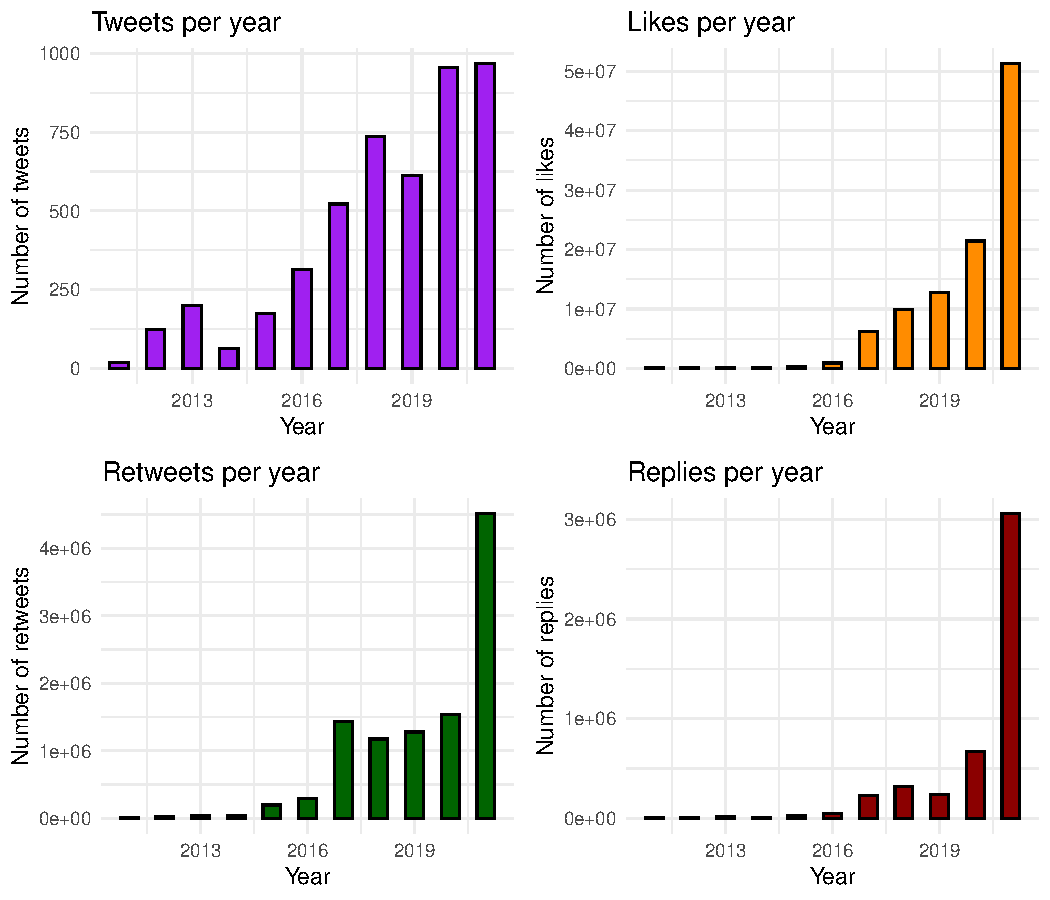
\includegraphics{Trial1_files/figure-latex/fi1s-1.pdf}
\caption{\label{fig:fig1}Elon's twitter interaction over time}
\end{figure}

\hypertarget{activty-of-crypto-related-tweets}{%
\subsubsection{Activty of crypto-related
tweets}\label{activty-of-crypto-related-tweets}}

In this section we want to compare how Elon Musk's audience react to
different type of tweets containing respectevely words related only to
\emph{dogecoin}, \emph{Bitcoin} and \emph{cypto}. As in the first
section, we use the \emph{number of likes}, \emph{number of retweets}
and \emph{number of replies} as proxy to popularity and high network
activity more generally. The first two categories are the most popular,
and between the two BTC-related tweets generate slightly more
interaction, coherently with the central importance that Bitcoin has in
the crypto scenario. The third category seems less ``popular'' but this
is only due to the specific address to certain currencies by the Tesla's
CEO.

\begin{figure}
\centering
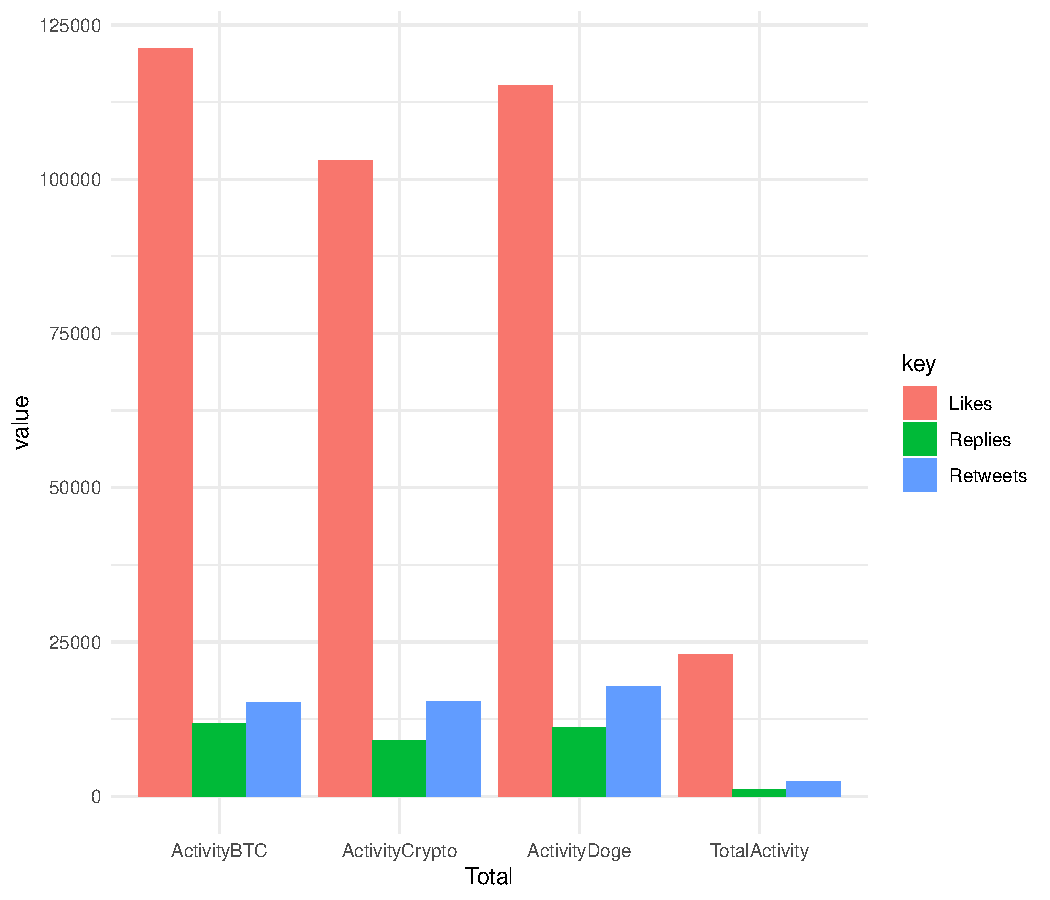
\includegraphics{Trial1_files/figure-latex/fig2-1.pdf}
\caption{\label{fig:fig2}Crypto-related content interaction}
\end{figure}

\hypertarget{when-elon-musks-tweets-investors-listen}{%
\subsection{When Elon Musks tweets, investors
listen}\label{when-elon-musks-tweets-investors-listen}}

Once quantified Elon Musk's influence, it is essential to understand the
extent of this influence on the cryptomarket. Which is the width of
Bitcoin price volatility once a crypto-related tweets is published? We
managed to extract the tweets which only cointained the words
\emph{bitcoin} and \emph{crypto} and connected their time-stamp to the
Bitcoin market capitalization trend. The pink points on the graphic
represent the moment in time when a crpyto-related tweet was published:
there is clear evidence suggesting a relationship between the Bitcoin
volatility and Musk's trend however, it is still unclear at this stage
whether it's Elon Musk's direct influence on Bitcoin price change or the
other way round. It cannot be assessed a clear causality relatioship.
This issue will be further addressed in this paper.

\begin{figure}
\centering
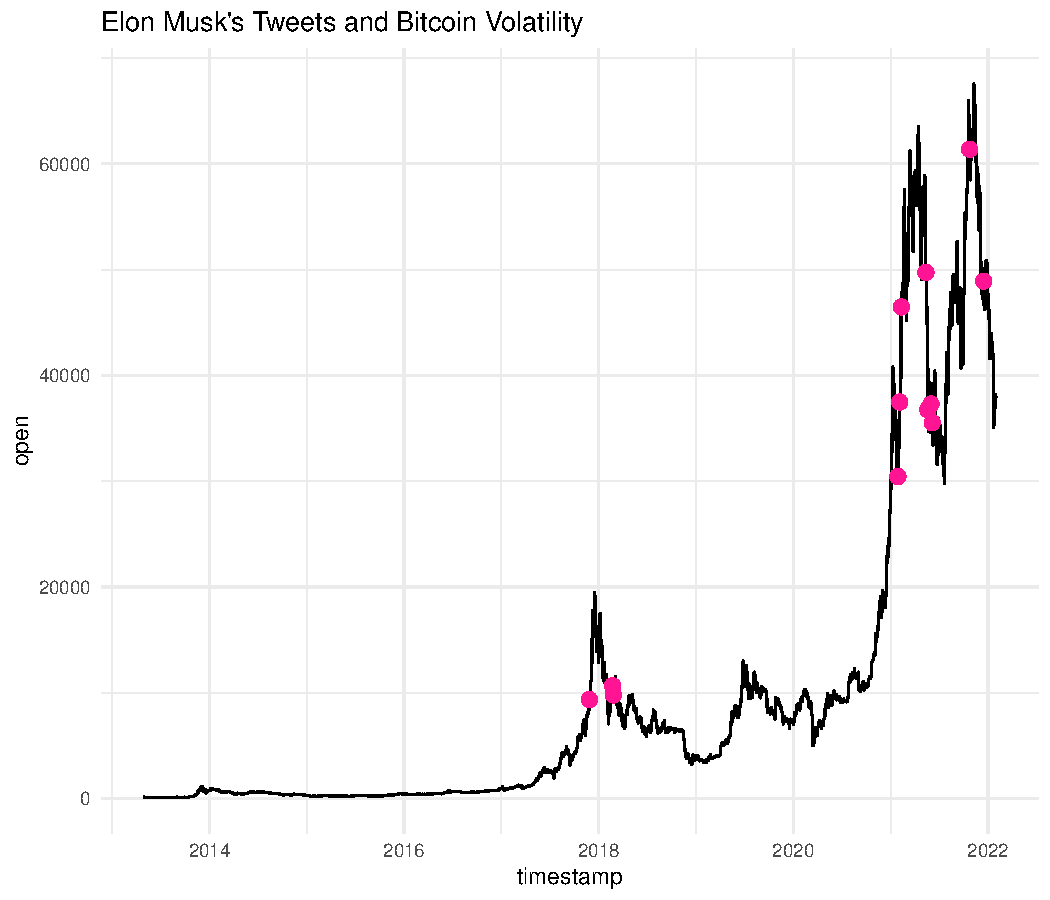
\includegraphics{Trial1_files/figure-latex/fig3-1.pdf}
\caption{\label{fig:fig3}BTC price compared with crypto-related tweets'
date}
\end{figure}

\hypertarget{sentiment-analysis-model-i}{%
\subsection{Sentiment Analysis : Model
I}\label{sentiment-analysis-model-i}}

While the market may interpret Musk's tweets about Tesla as ``accurate
news'', his tweets about cryptocurrency at least to some degree
represent moods or personal sentiment. In this section we want to
further analyze the nature of this sentiments, the most frequent words
and the emotions associated to them.

The graph below shows the most used word and their frequency. It appears
that the three most used words are \emph{amp}, \emph{tesla} and
\emph{will}. We find the presence of more than 600 words for the firsts
two, while more than 500 words for the latter. It goes without saying
that we expected \textbf{tesla} to be one of the most frequent word in
Musk's tweet, and our interpretation of the word \textbf{will} lies in
that this verb shows his strong willingness and decisive, goal-oriented
character as well as his inclination towards the future sustained by
visionary statements. It can be less clear why \textbf{amp} is among the
most frequent word, therefore we opted for a further explanation.

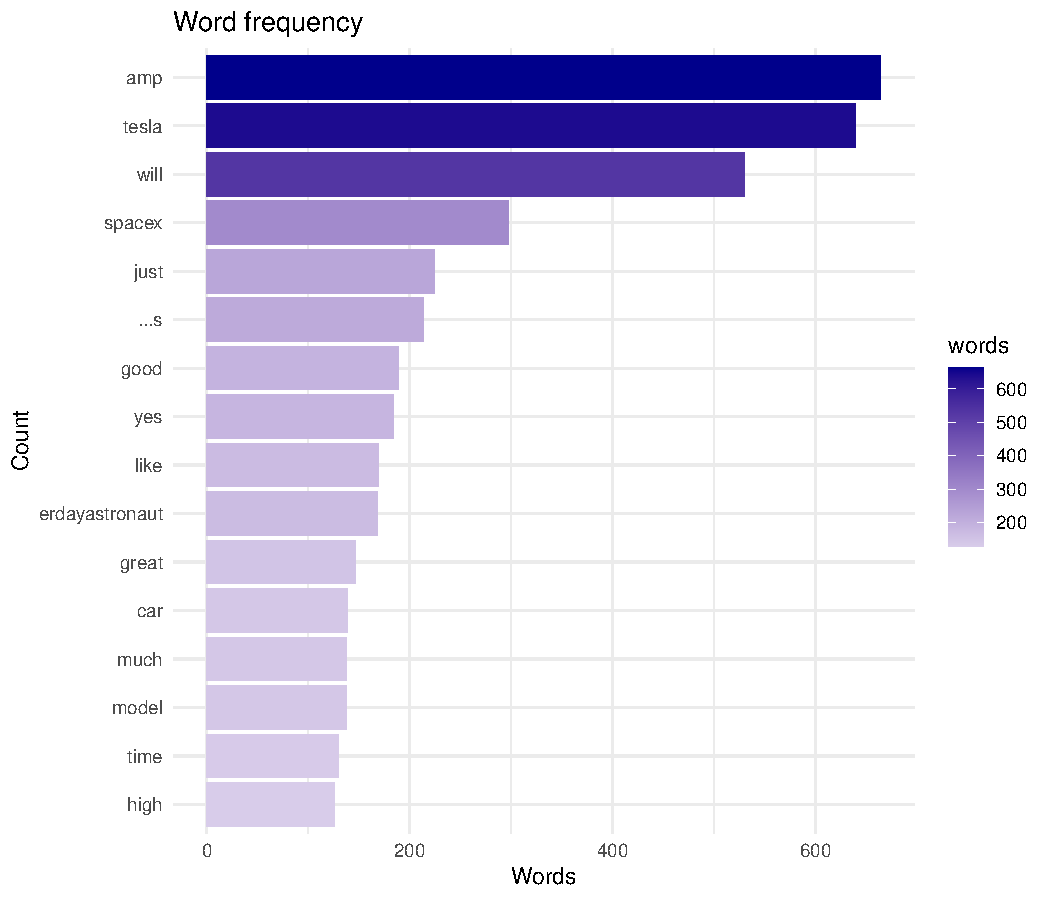
\includegraphics{Trial1_files/figure-latex/fig4-1.pdf} \emph{AMP}

Amp is a universal collateral token designed to facilitate fast and
efficient transfers for any real-world application. When using Amp as
collateral, transfers of value are guaranteed and can settle instantly.
While the underlying asset reaches final settlement, a process that can
take anywhere from seconds to days, Amp is held in escrow by a
collateral manager. Once the transaction successfully settles, the Amp
collateral is released and made available to collateralize another
transfer. Amp exists to serve as universal collateral for anyone and any
project. (\emph{Source {[}(\url{https://docs.amptoken.org/}){]}} ).
Besides being a collateral for individuals and DeFi platforms, Amp is
used as a collateral for payment networks: Flexa uses Amp to enable
instant, fraud-free payments to merchants across its digital payment
network. Apps that integrate Flexa stake Amp to ensure all payments can
be settled in real-time regardless of the asset or protocol used. Since
AMP Token was to be integrated with Tesla's payment rail for crypto, it
is understandable why it's been one of the most tweeted words by Elon
Musk, being this news shocking the crypto-lovers panorama and the future
of Tesla. The news of Tesla about the willing to accept crypto as
payments and the investment in over 1.5 BLN USD in Bitcoin (February
2021), made the price of Bitcoin to skyrocket. On the other hand, a
plethora of enviromental activists opposed this decision due to the high
levels of electric energy which are used to mine and sustain the crypto
network and highlighted the controversial nature of the Tesla CEO's
choice: this led Elon Musk to no longer accept payments in Bitcoin. The
impact on the crypto-currency value has been devastating has shown in
the following graphic showing once again, how much ``investors listen to
Elon Musk''.

image: 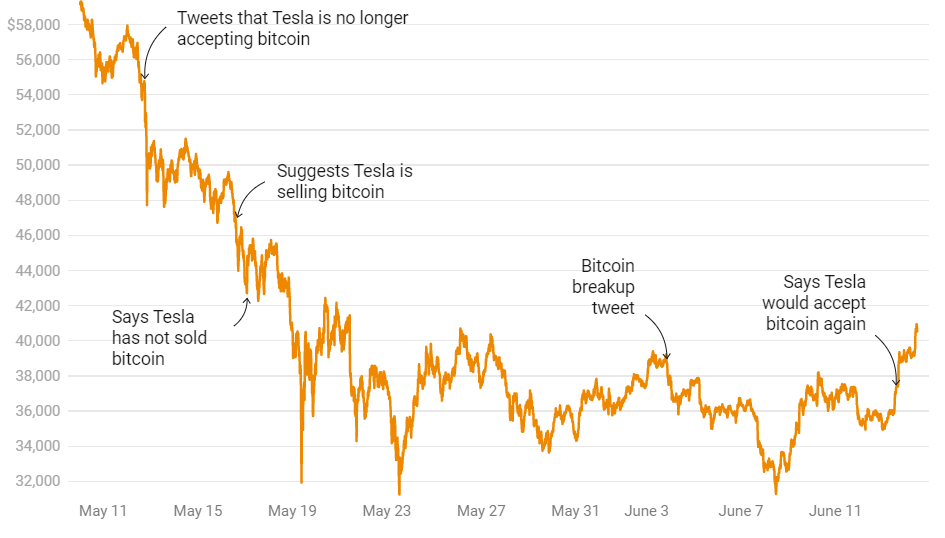
\includegraphics{events_image.jpg}

Here follows a wordcloud which helped us to visualize the most frequent
words in Elon Musk's tweets. The higher the word's size displayed, the
most frequent the word would appear in his tweets.

\begin{figure}
\centering
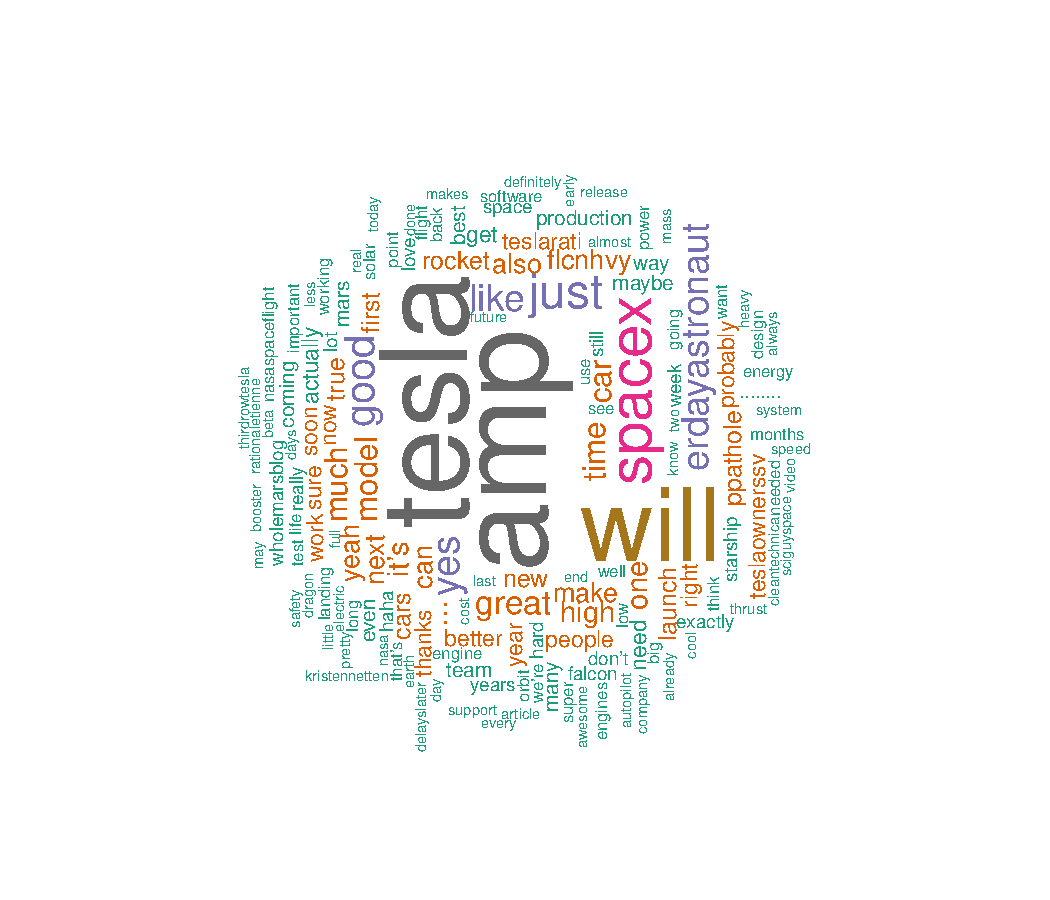
\includegraphics{Trial1_files/figure-latex/fig5-1.pdf}
\caption{\label{fig:fig5}Wordcloud of most commons words}
\end{figure}

\hypertarget{sentiment-scores-and-density}{%
\subsubsection{Sentiment scores and
density}\label{sentiment-scores-and-density}}

Based on the following results of the Sentiment Analysis of Elon Musk's
tweets, it appears clear that \emph{positive}, \emph{trust} and
\emph{anticipation} are the most frequent emotions. This result is
perfectly coherent with the visionary Tesla and SpaceX CEO's
personality: his hunger for innovative , out-of-the-box solutions; his
continuous positive and confident approach towards insurmountable
problems such as ``taking the human race to Mars'', conceiving re-usable
rockets disrupting space industry, as well as ``changing the world's
concept of driving through electric autonomous driven vehicle'' and many
others clearly embeds those emotions.

\begin{verbatim}
##   anger anticipation disgust fear joy sadness surprise trust negative positive
## 1     2            1       1    2   1       1        1     1        2        1
## 2     0            0       0    0   0       0        0     0        0        1
## 3     1            1       2    2   0       2        0     1        2        1
## 4     0            0       0    0   0       0        0     1        0        1
## 5     0            1       0    0   1       0        0     3        0        3
## 6     0            0       0    0   0       0        0     0        0        0
\end{verbatim}

\begin{figure}
\centering
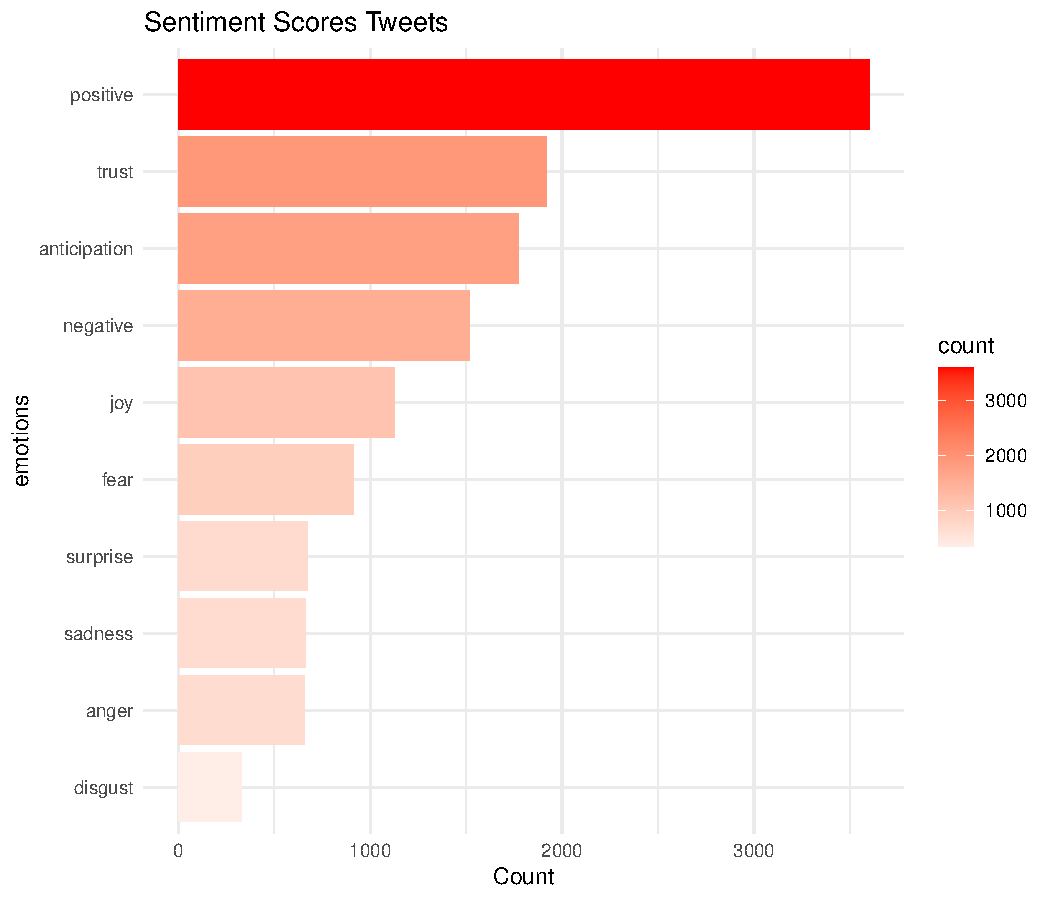
\includegraphics{Trial1_files/figure-latex/fig6-1.pdf}
\caption{\label{fig:fig6}Sentiment scores of Elon's tweets}
\end{figure}

Another important result is outlined by the following graphs. It shows
the density of sentiment: as it can be noticed it follows a normal-like
distribution (\(\mu = 0.18\), \$\sigma = 0.36 \$), slightly positevely
skewed. This result is line with the previous results, highlighting the
positive polarity of the sentiments. Here follows a brief statistical
summary of the density plot, followed by the plot itself.

\begin{verbatim}
##          Statistical summary sentiment
## Mean                        0.18242245
## Sd                          0.35932881
## IQR                         0.45907962
## Skewness                   -0.04752713
## Kurtosis                    0.79887814
\end{verbatim}

\begin{figure}
\centering
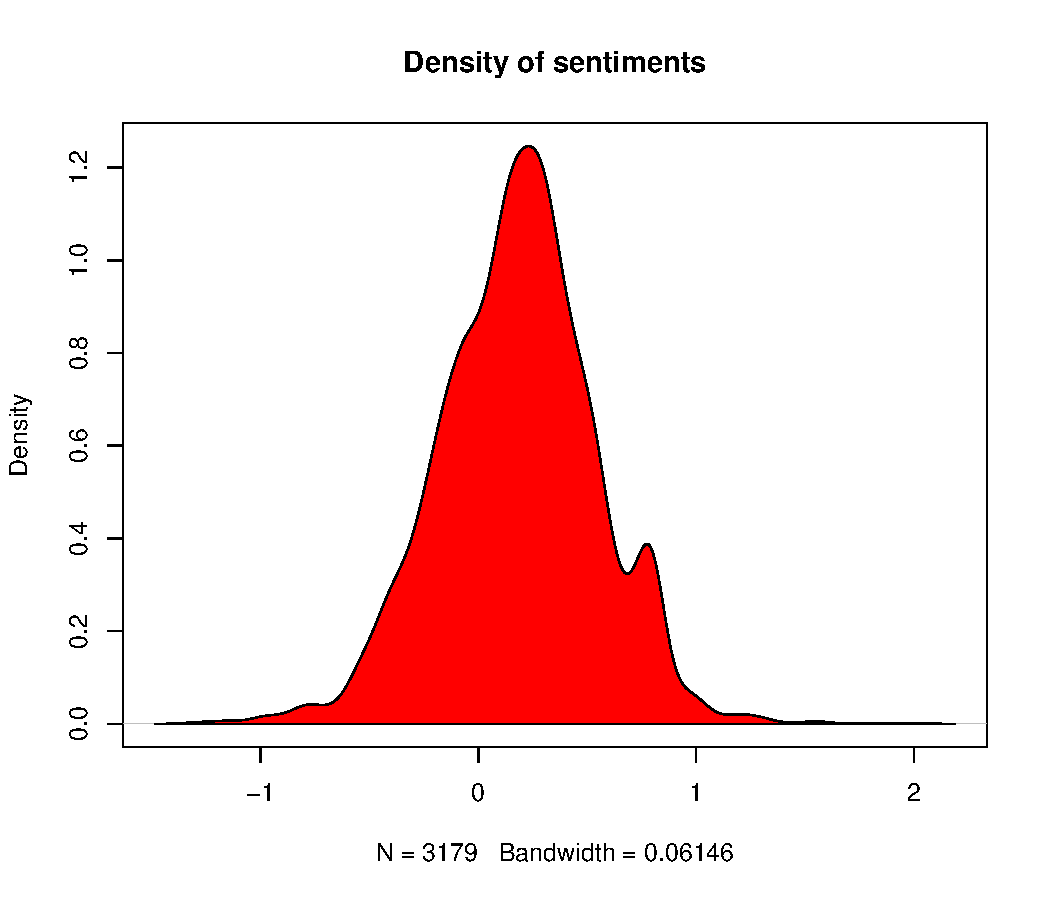
\includegraphics{Trial1_files/figure-latex/fig7-1.pdf}
\caption{\label{fig:fig7}density of polarity scores}
\end{figure}

\hypertarget{emotions-at-the-sentence-level}{%
\subsubsection{Emotions at the sentence
level}\label{emotions-at-the-sentence-level}}

The following analysis detects the rate of emotion at the sentence
level. This method uses a simple dictionary lookup to find emotion words
and then compute the rate per sentence. The emotion score ranges between
0 (no emotion used) and 1 (all words used were emotional). Once again,
this result is in line with the previous ones, showing how positive
emotions such as joy, trust and anticipation are predominant. Please
note that the suffix *\_negated* indicates the opposite of the reference
emotions, which appears to be consistently absent in relation to any
emotion.

\begin{figure}
\centering
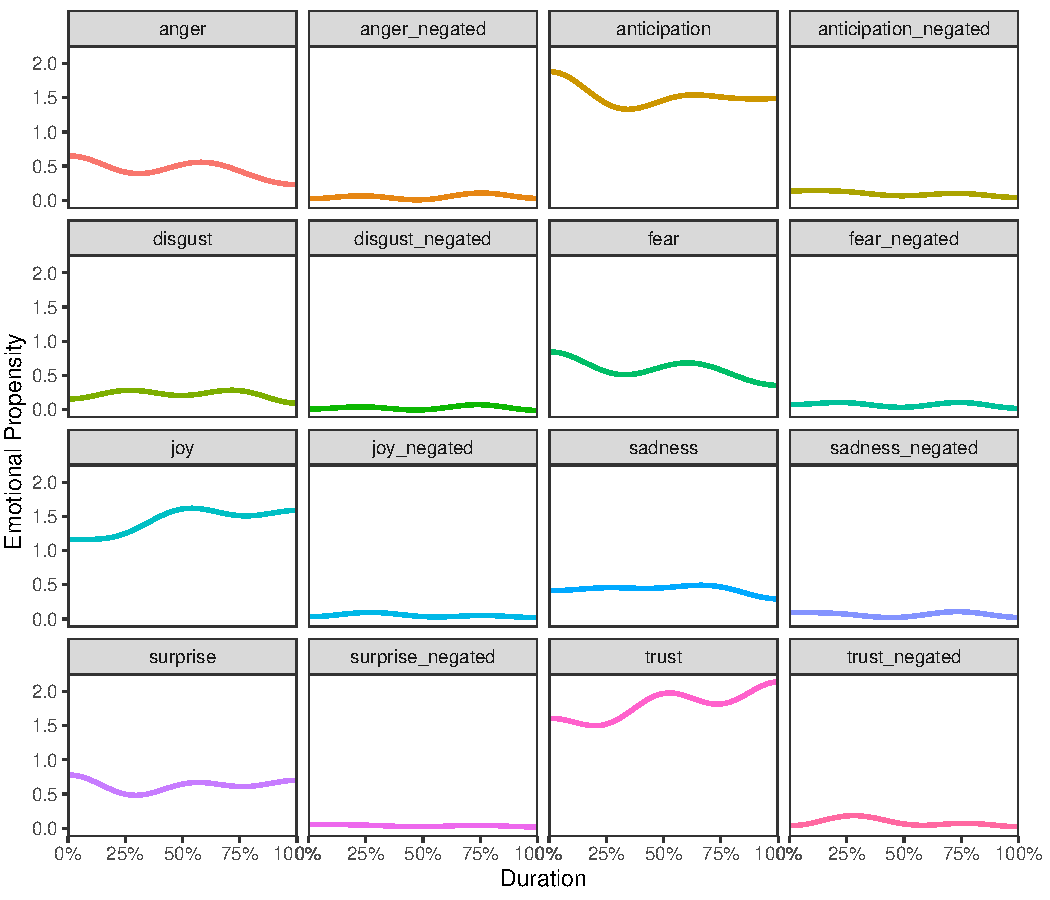
\includegraphics{Trial1_files/figure-latex/fig8-1.pdf}
\caption{\label{fig:fig8}plot of Emotions}
\end{figure}

\hypertarget{subsetting-sentiment-from-jan-2020-without-amp-word-sentiment-model-ii}{%
\subsection{Subsetting sentiment from Jan 2020 without ``AMP'' word:
Sentiment model
II}\label{subsetting-sentiment-from-jan-2020-without-amp-word-sentiment-model-ii}}

Once obtained solid result for the entire dataset of tweets ranging from
year 2011 to 2021, it is interesting to compare those with new results
coming from a subset of the selected time frame. We believe it is an
interesting way to assess our results' coherence and a further
investigation into the ``popular'' period of Elon Musk. Furthermore we
believe the most used word, i.e \emph{AMP}, should be removed in order
to assess whether the absence of this word could influence the final
output. In a programatic approach, we apply the same methods, codes and
considerations of the previous section on a different subset of data.

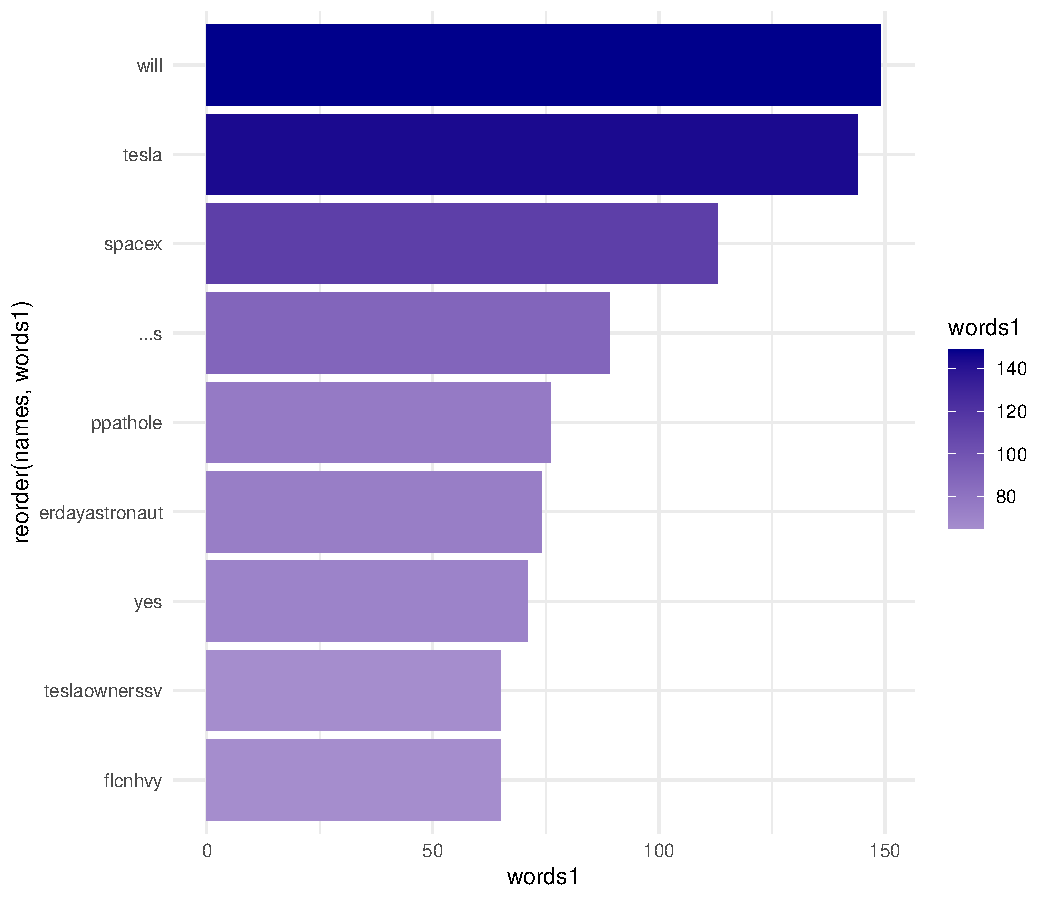
\includegraphics{Trial1_files/figure-latex/fig9-1.pdf} This primary
result is in line with the previous ones, once again the two most used
words are \emph{tesla}, \emph{will} and \emph{spacex}. The frequency of
each word is compared in the chart above. We proceed displaying a
wordcloud, in order to have an eye-friendly visualization of the word
frequency in this new subset of data.

\begin{figure}
\centering
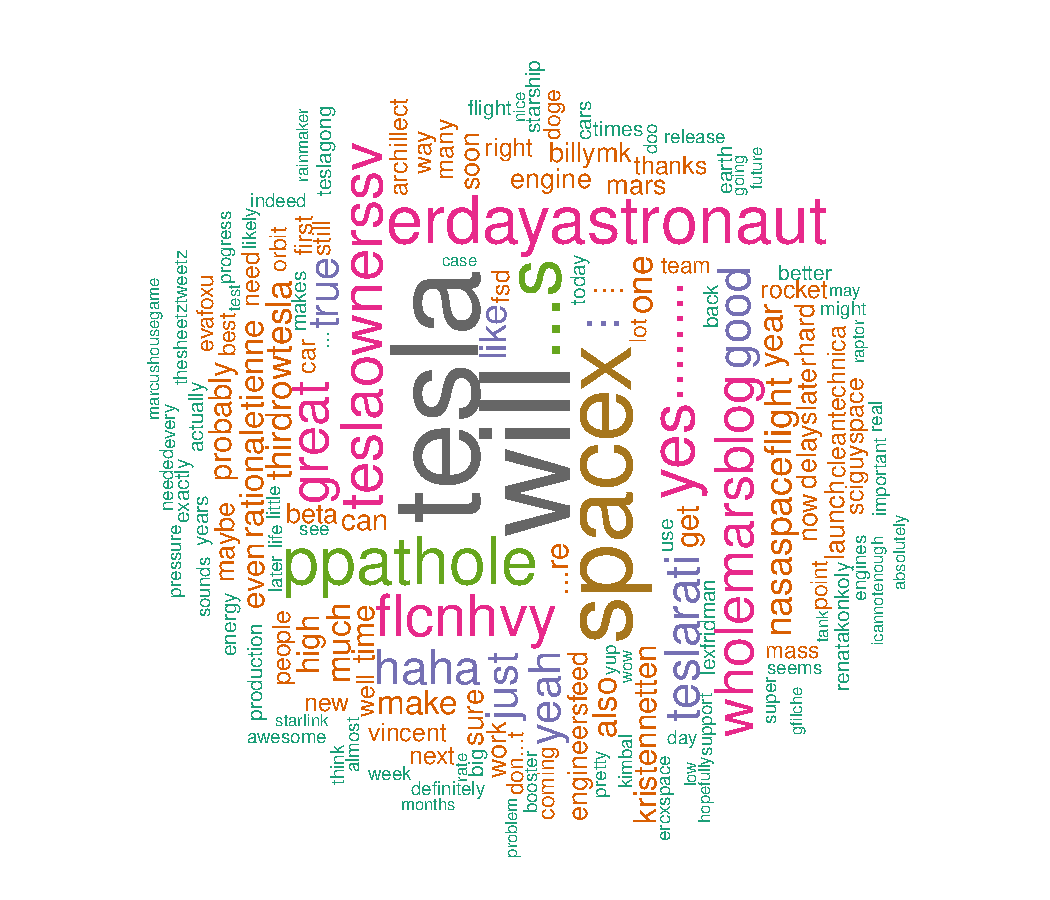
\includegraphics{Trial1_files/figure-latex/fig10-1.pdf}
\caption{\label{fig:fig10}Wordcloud of Elon's tweets resampled}
\end{figure}

\hypertarget{sentiment-scores-and-density-1}{%
\subsubsection{Sentiment scores and
density}\label{sentiment-scores-and-density-1}}

Consistently with the previous results, the \emph{Muskanian} influence
is still positive with the most frequent sentiments of \emph{positive},
\emph{anticipation} and \emph{trust}.

\begin{figure}
\centering
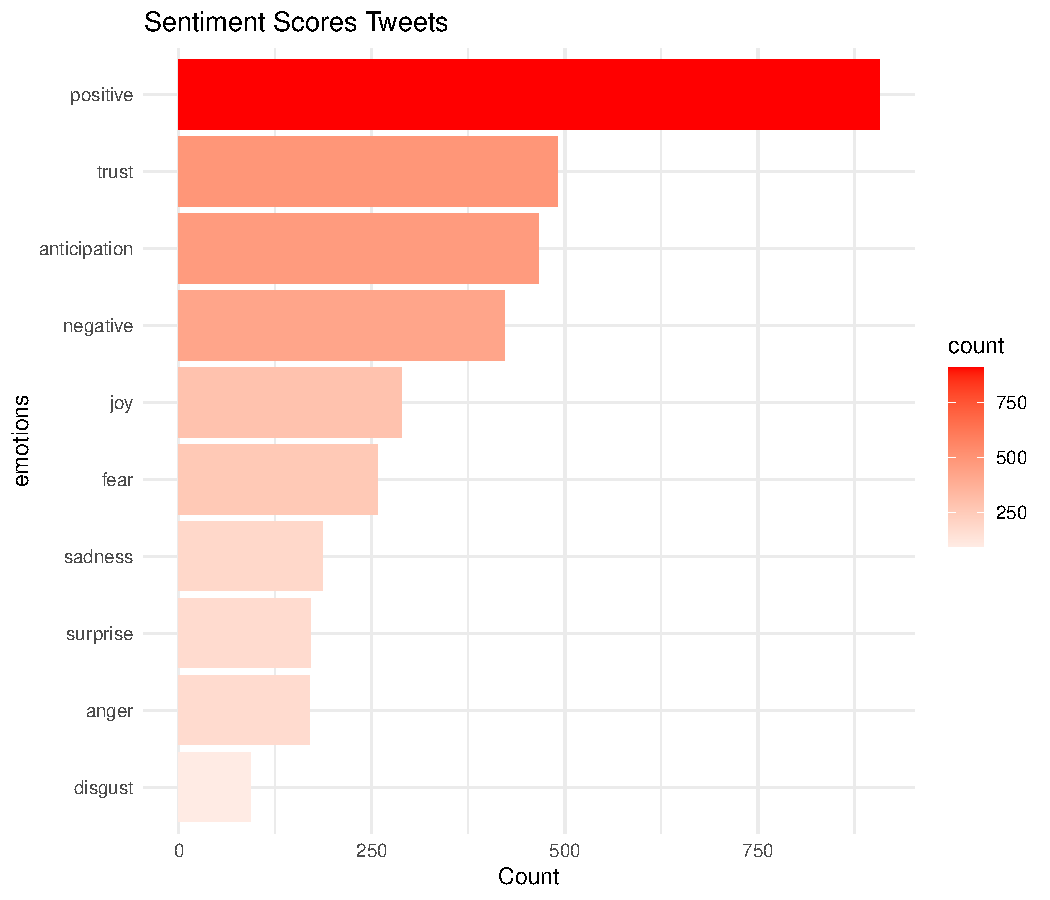
\includegraphics{Trial1_files/figure-latex/fig11-1.pdf}
\caption{\label{fig:fig11}Sentiment Score of Elon's tweets resampled}
\end{figure}

The density of sentiment is slightly different from the first one: as it
can be noticed it still follows a normal-like distribution
(\(\mu = 0.19\), \$\sigma = 0.39 \$), slightly positevely skewed. This
result is line with the previous results, stating the even more positive
polarity of the sentiments in the new timeframe. A brief statistical
summary of the new density plot compared to the previous one is
displayed. A new density plot can be found in the chart below.

\begin{verbatim}
## New names:
## * `Statistical summary sentiment` -> `Statistical summary sentiment...1`
## * `Statistical summary sentiment` -> `Statistical summary sentiment...2`
\end{verbatim}

\begin{verbatim}
##          Sentiment model I Sentiment model II
## Mean             0.1981359         0.18242245
## Sd               0.3859845         0.35932881
## IQR              0.5028519         0.45907962
## Skewness        -0.1307537        -0.04752713
## Kurtosis         0.6063917         0.79887814
\end{verbatim}

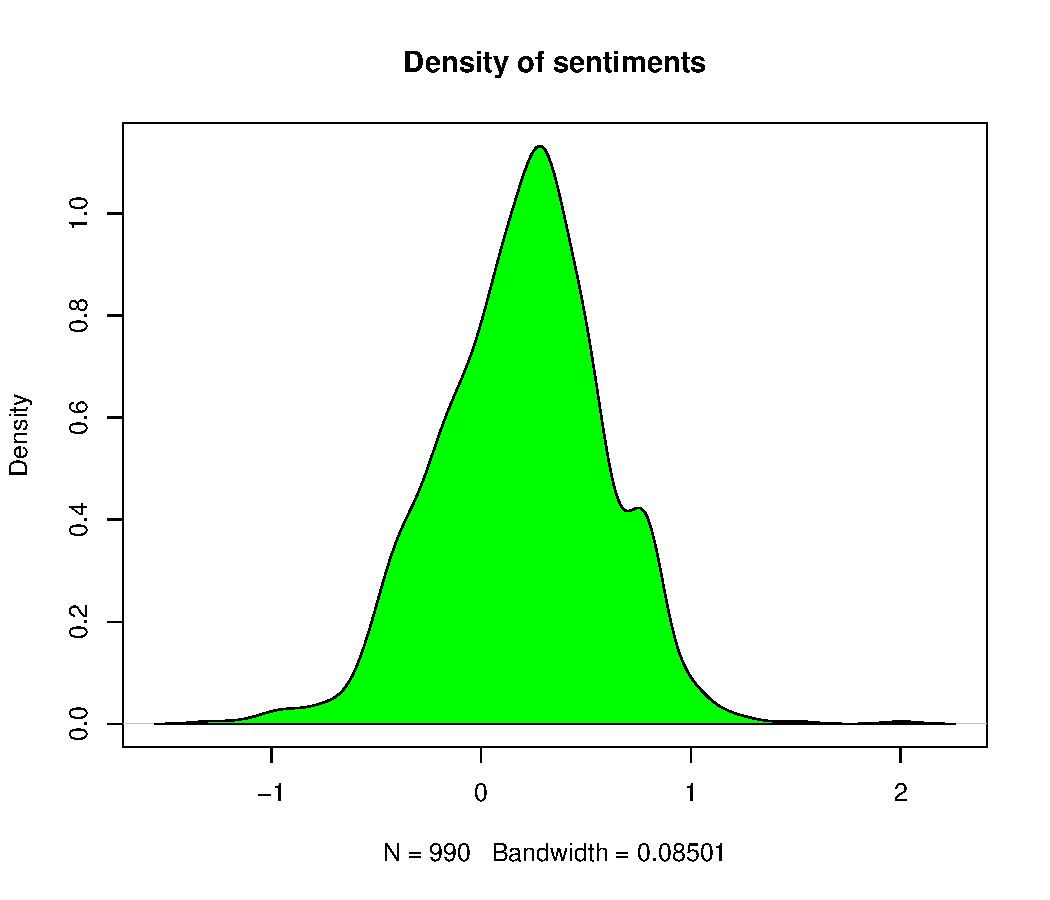
\includegraphics{Trial1_files/figure-latex/fig12-1.pdf} The chart below
shows an overall overlapping with the previous result. Still positive
sentiment of \emph{anticipation}, \emph{joy} and \emph{trust} are the
most frequent. However, the sentiment of \emph{trust} is more volatile,
and there is a slight decrease in the negative sentiment of \emph{fear}.
This slight but still relevant change can be interpreted in a different
context than the one of model I: the audience has become more educated
and informed about the phenomenon of crypto-currencies as well as more
critical towards the Tesla CEO's tweets, who sometimes has been accused
more intensively of market manipulation (however without losing
popularity or positive appeal). In conclusion, the Muskanian audience
still listen to him and trust him, simply with more critical sense which
makes the \emph{trust} sentiment to be more volatile and the \emph{fear}
sentiment lower.

\begin{figure}
\centering
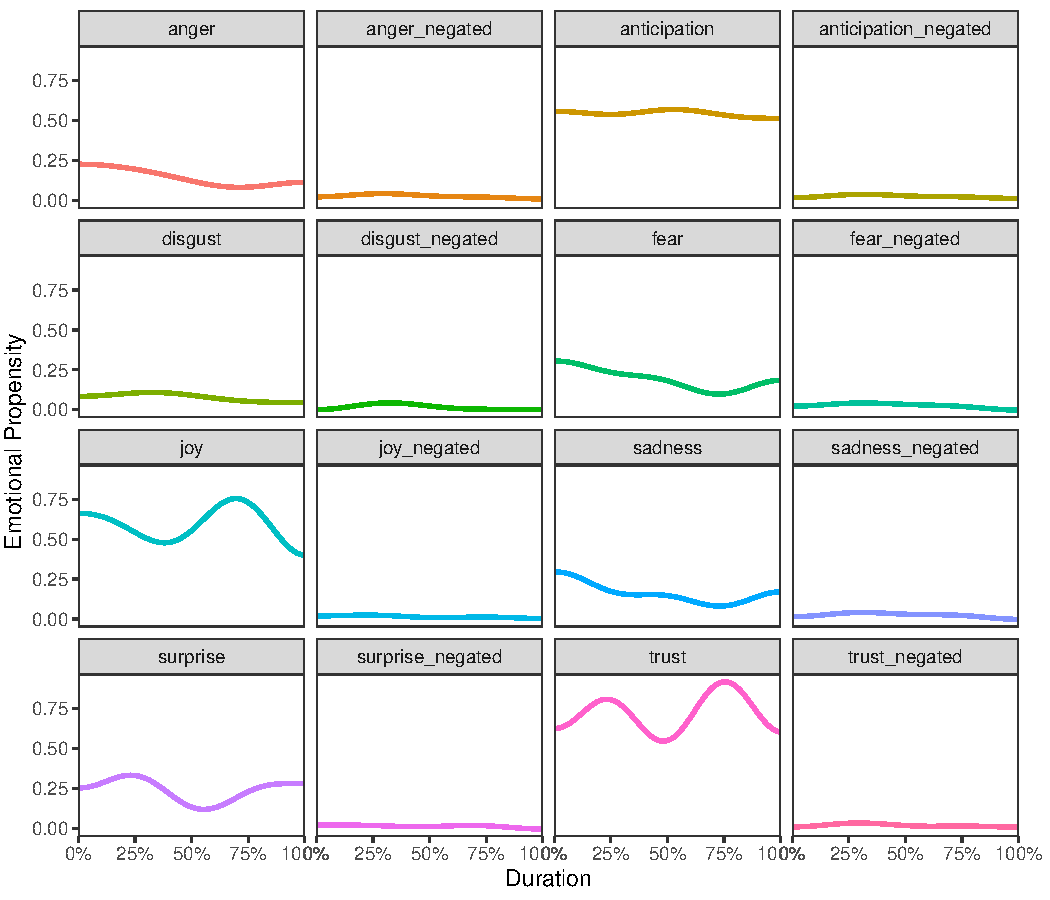
\includegraphics{Trial1_files/figure-latex/fig13-1.pdf}
\caption{\label{fig:fig13}Emotion's Plot of Elon's tweets resampled}
\end{figure}

\hypertarget{testing-for-stationarity-1}{%
\subsection{Testing for stationarity}\label{testing-for-stationarity-1}}

In this section we show the results obtained when testing for Bitcoin
trend stationarity. We recall the hypothesis:

\emph{Null Hypothesis (H0} : Null hypothesis of the test is that the
time series can be represented by a unit root that is not stationary.
\emph{Alternative Hypothesis (H1)}: Alternative Hypothesis of the test
is that the time series is stationary. The following plot, represent our
study focus.

\hypertarget{autocorrelation-function}{%
\subsubsection{Autocorrelation
Function}\label{autocorrelation-function}}

The autocorrelation function (ACF) defines how data points in a time
series are related, on average, to the preceding data points (Box,
Jenkins, \& Reinsel, 1994). In other words, it measures the
self-similarity of the signal over different delay times. An
autocorrelation plot shows the value of the autocorrelation function
(ACF) on the vertical axis. It can range from --1 to 1. We use
autocorrelation plot to assess wether the elements of a time series
randomly oscilates around zero.

Our first attempt without any transformation gives the following result,
which shows consistent non-stationarity.
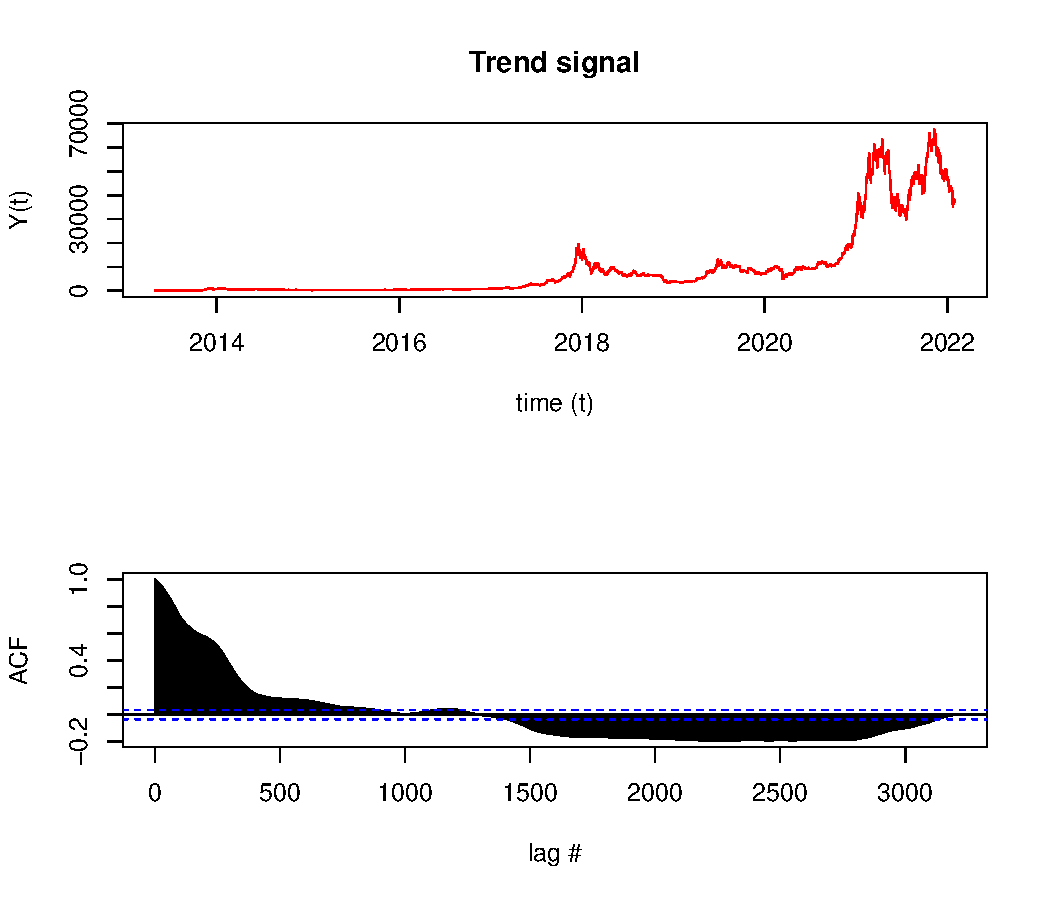
\includegraphics{Trial1_files/figure-latex/fig14-1.pdf} We proceed by
applying an Augmented Dickey--Fuller (ADF) t-statistic test for unit
root: in statistics and econometrics, an augmented Dickey--Fuller test
(ADF) tests the null hypothesis that a unit root is present in a time
series sample. The alternative hypothesis is different depending on
which version of the test is used, but is usually stationarity or
trend-stationarity. It is an augmented version of the Dickey--Fuller
test for a larger and more complicated set of time series models. The
augmented Dickey--Fuller (ADF) statistic, used in the test, is a
negative number. The more negative it is, the stronger the rejection of
the hypothesis that there is a unit root at some level of confidence.
Our result clearly shows a non-stationarity due to the high p-value
(\textgreater0.5).

In order to go from non-stationarity to stationarity different
techniques can be used. We first attempt in utilising logaritmic
transformation: such transformtion can help to stabilise the variance of
a time series. We apply the ADF test, still obtaining a non
statistically relevant result, even though the p-value has decreased to
0.46.

\begin{figure}
\centering
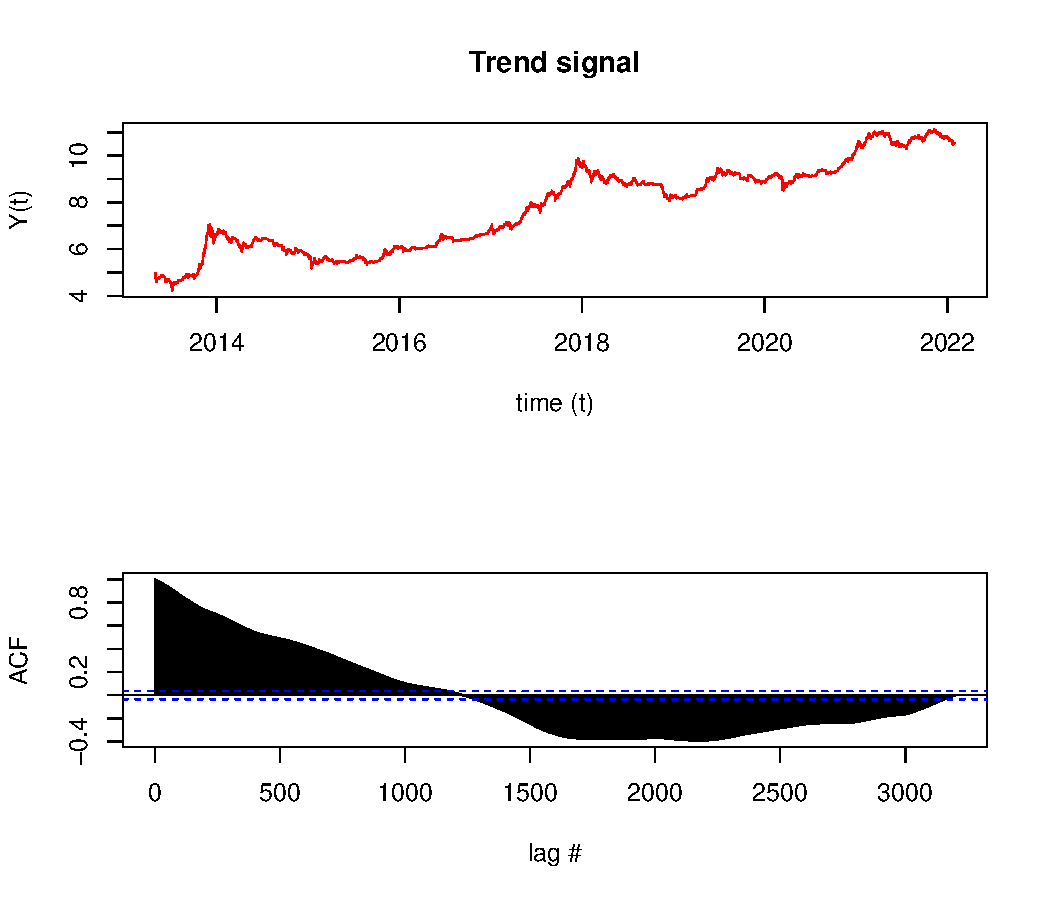
\includegraphics{Trial1_files/figure-latex/fig15-1.pdf}
\caption{\label{fig:fig15}LogBitcoin's trend and ACF function}
\end{figure}

Differencing log values can help stabilise the mean of a time series by
removing changes in the level of a time series, and therefore
eliminating (or reducing) trend and seasonality. We attempt to use this
transformation obtaining satisfing results. Indeed, the following plot
shows how the trend has been removed and stationarity is obtained.

\begin{figure}
\centering
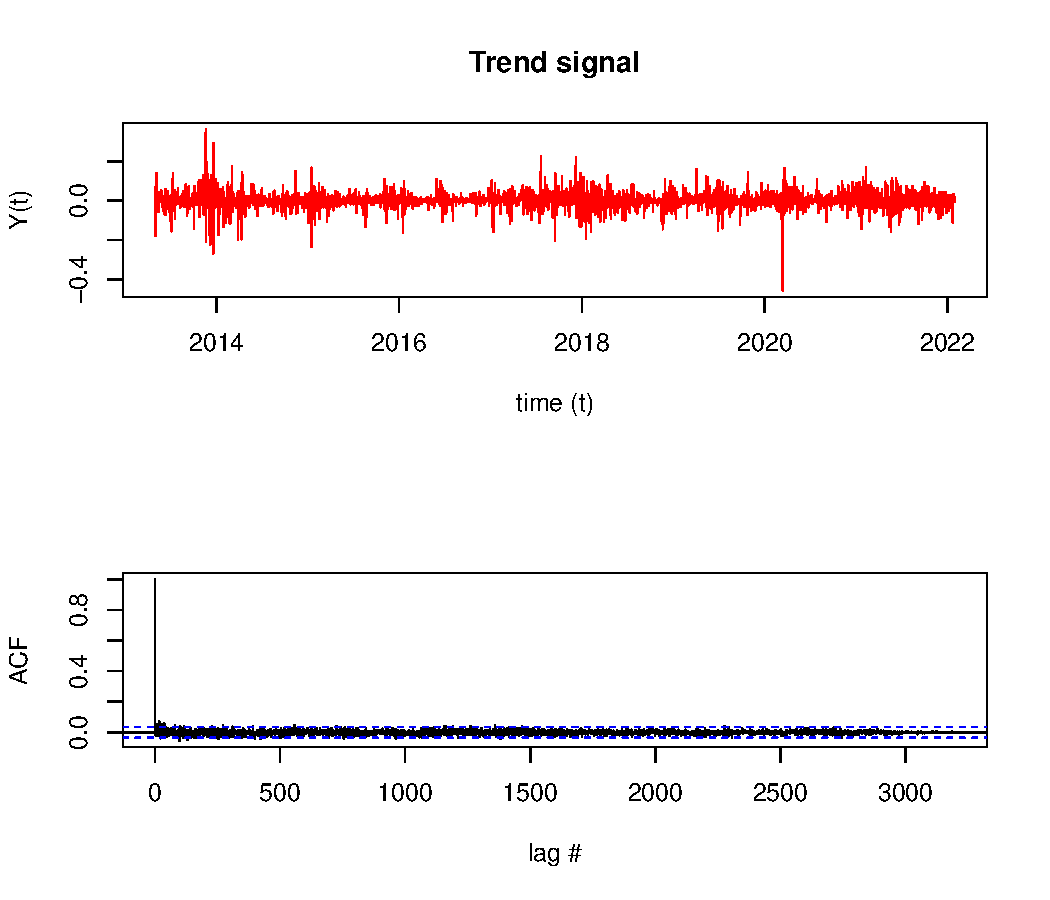
\includegraphics{Trial1_files/figure-latex/fig16-1.pdf}
\caption{\label{fig:fig16}Differences of LogBitcoin's trend and ACF
function}
\end{figure}

We conduct the ADF test to confirm our results: p-value is now 0.01
(highly significant) and we can assess that the log difference of the
elements of the time series result to be non-stationary.

This means that bitcoin volatility is random, not influenced by Elon
Musk's tweets. This is a core finding of our study.

try to find change points in the data, I use diff for now not sure tho

\begin{Shaded}
\begin{Highlighting}[]
\NormalTok{m\_binseg }\OtherTok{\textless{}{-}} \FunctionTok{cpt.mean}\NormalTok{(logdiff, }\AttributeTok{penalty =} \StringTok{"BIC"}\NormalTok{, }\AttributeTok{method =} \StringTok{"BinSeg"}\NormalTok{, }\AttributeTok{Q =} \DecValTok{15}\NormalTok{)}

\FunctionTok{plot}\NormalTok{(m\_binseg, }\AttributeTok{type =} \StringTok{"l"}\NormalTok{, }\AttributeTok{xlab =} \StringTok{"Index"}\NormalTok{, }\AttributeTok{cpt.width =} \DecValTok{4}\NormalTok{)}
\end{Highlighting}
\end{Shaded}

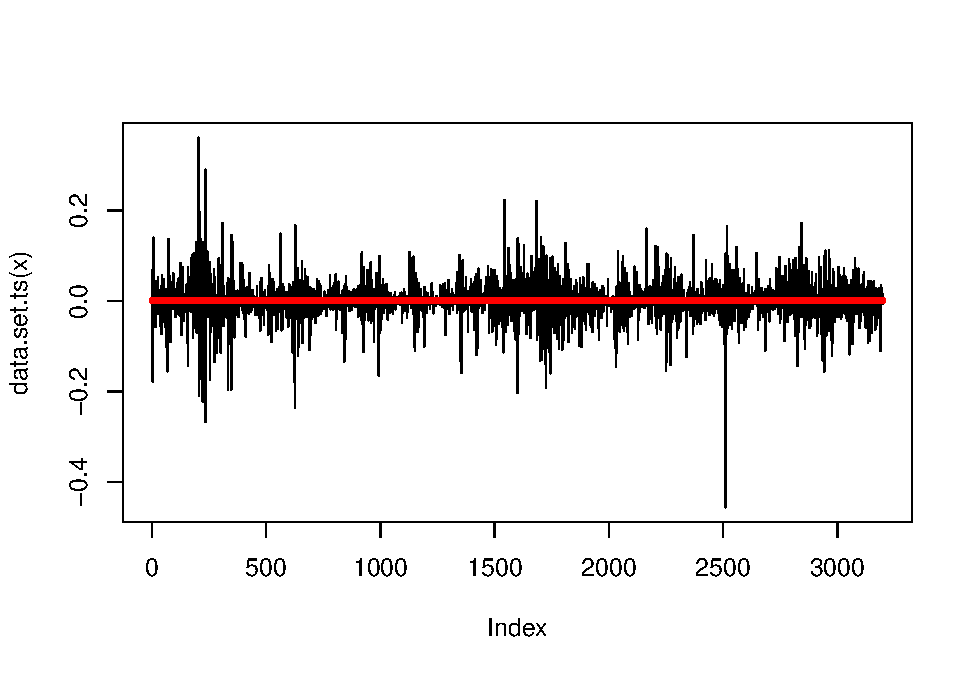
\includegraphics{Trial1_files/figure-latex/include==FALSE-1.pdf}

\begin{Shaded}
\begin{Highlighting}[]
\CommentTok{\#all the changes happen from 2750 onwards approx, try to subset plot}
\NormalTok{m\_binseg }\OtherTok{\textless{}{-}} \FunctionTok{cpt.mean}\NormalTok{(logdiff[}\DecValTok{2750}\SpecialCharTok{:}\DecValTok{3199}\NormalTok{], }\AttributeTok{penalty =} \StringTok{"None"}\NormalTok{, }\AttributeTok{method =} \StringTok{"BinSeg"}\NormalTok{, }\AttributeTok{Q =} \DecValTok{15}\NormalTok{)}
\end{Highlighting}
\end{Shaded}

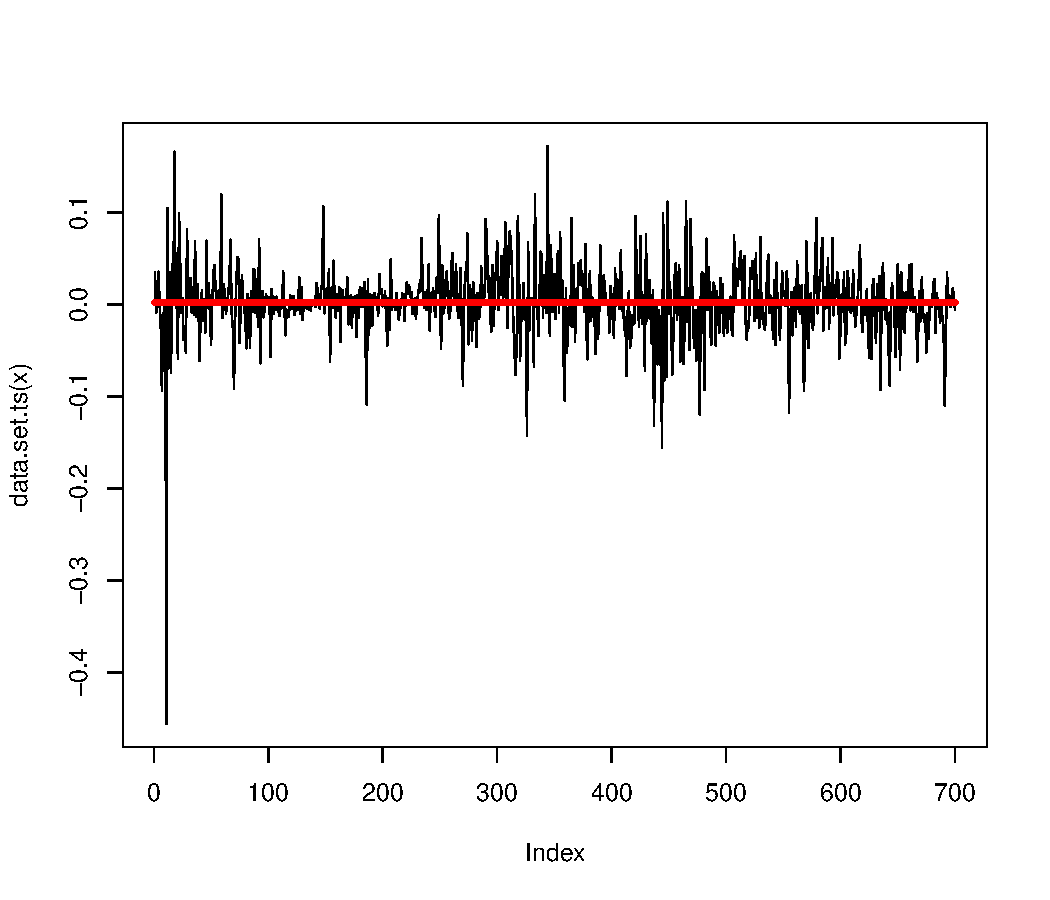
\includegraphics{Trial1_files/figure-latex/fig17-1.pdf} tried with
differend methods (segmented neighbour and PELT, but Binseg most
effective):

Those were only taking into consideration the mean, let's see the
results for mean and variance all together

In the chart below a deep investigation regarding the potential linkage
between Bitcoin volatility and Musk's tweet has been conducted. In blue
the \emph{breaking points} are highlighted, which are points in time
where the average value of the Bitcoin price undergoes a sudden change.
In purple we find highlighted when the crypto-related \emph{tweets} were
published. As we can notice, there is no correspondence or correlation
of the two variables: we cannot state that Musk's tweets influence
Bitcoin volatility, which is in-line with our previous result of
non-stationarity.

\begin{figure}
\centering
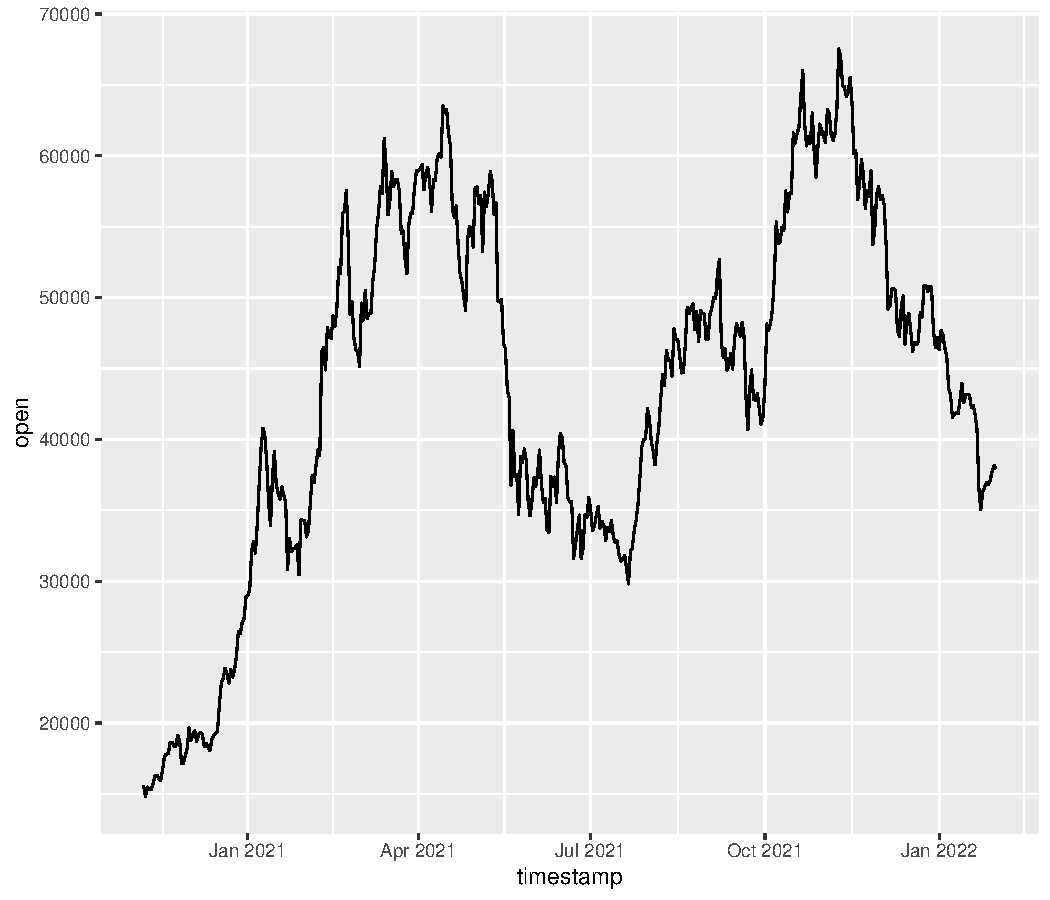
\includegraphics{Trial1_files/figure-latex/fig25-1.pdf}
\caption{\label{fig:fig25}Elon Musk's Tweets on Cryptos and LogBTC's
Changing Points Dates}
\end{figure}

\textless\textless\textless\textless\textless\textless\textless{} HEAD
Our findings are strenghtened by the confirming the previous result and
considerations for the Dogecoin cryptocurrency. We proceed in the same
way as before, analzying the trend signal and moving from
non-stationarity towards stationarity, as it can be seen in the results
below.

\begin{figure}
\centering
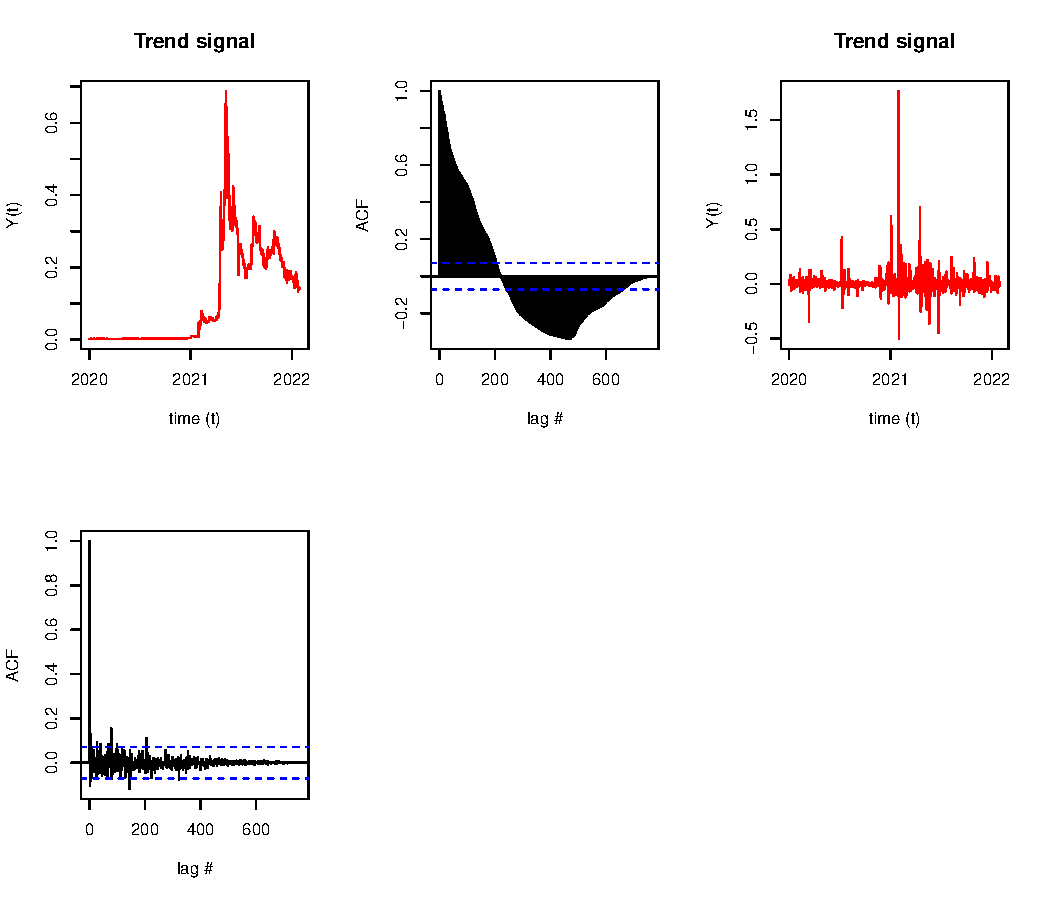
\includegraphics{Trial1_files/figure-latex/fig19-1.pdf}
\caption{\label{fig:fig19}Doge and Diff LogDoge trend with its
respective ACF}
\end{figure}

\begin{figure}
\centering
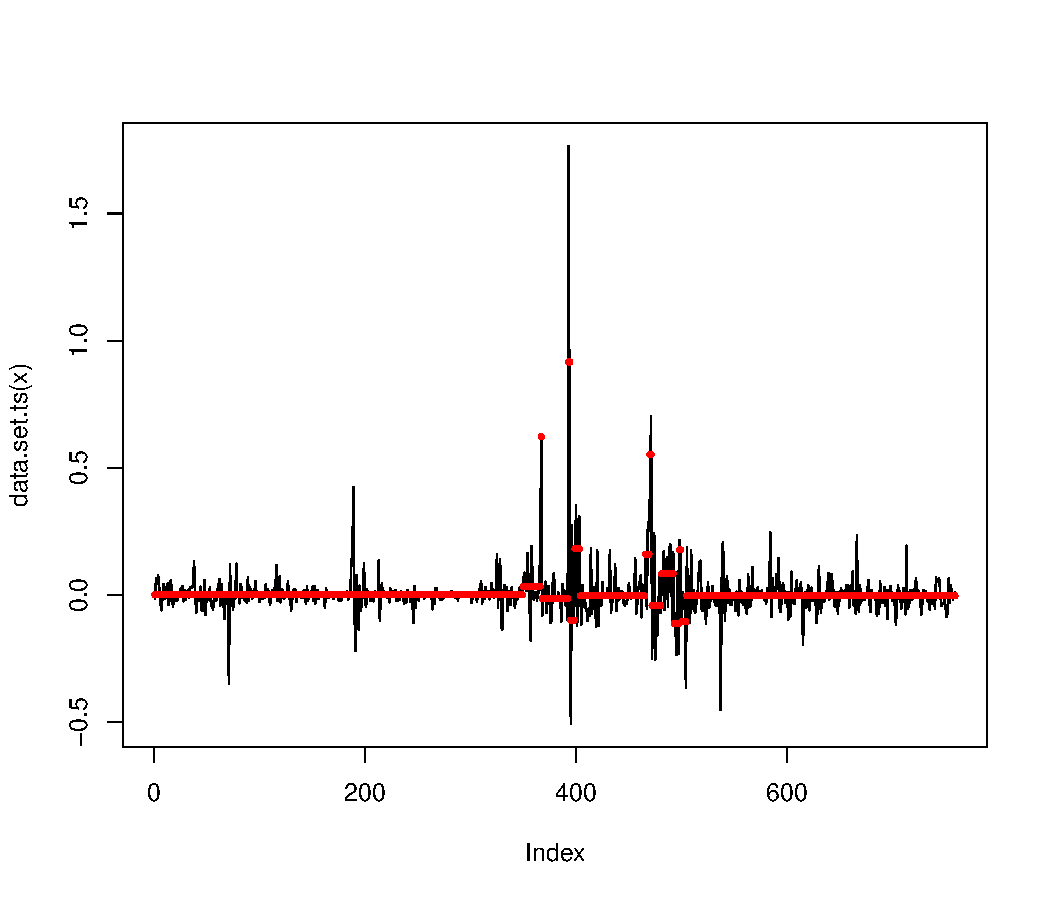
\includegraphics{Trial1_files/figure-latex/fig20-1.pdf}
\caption{\label{fig:fig20}Change point in differences of LogDoge}
\end{figure}

The breaking points versus tweet timestamp analysis on Dogecoin currency
confirms and strenghten our findings: there is no linkage between Musk's
tweet and the crypto-currency volatility.

\begin{figure}
\centering
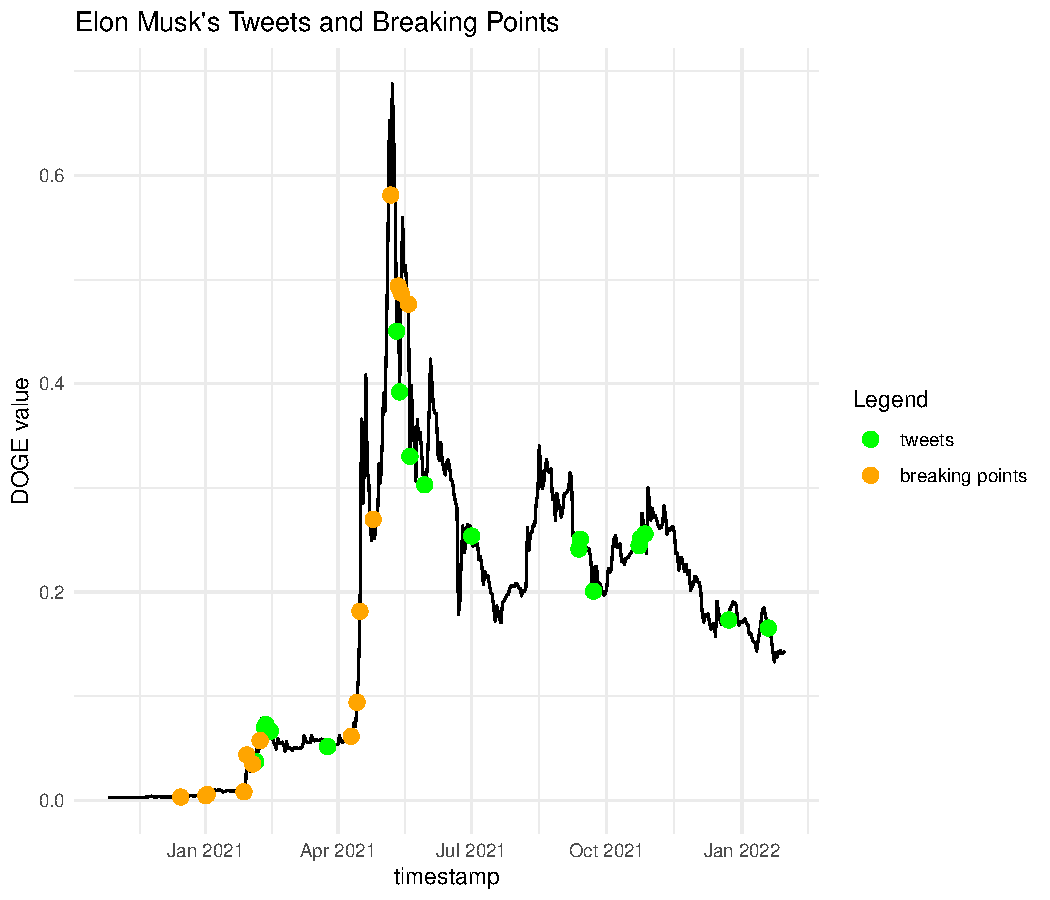
\includegraphics{Trial1_files/figure-latex/fig21-1.pdf}
\caption{\label{fig:fig21}Elon Musk's Tweets on Dogecoin and LogDoge's
Changing Points Dates}
\end{figure}

\hypertarget{conclusion}{%
\section{Conclusion}\label{conclusion}}

We have extracted a total of 4787 tweets containing 68676 words from
Elon Musk's twitter profile: we investigate the impact of 26 Twitter
events by Elon Musk on the trading volume and price of the
cryptocurrencies he comments on. Firstly we conducted a popularity
analysis, where the influencing power of the Tesla CEO's can be seen
skyrocketing throughout the years, especially after year 2016. A
sentiment approach has been adopted into investigating his
activity-related emotions, with an overall positive range of emotions
associated to it, as well as a frequency analysis on the most used words
and polarity analysis (Model I). A subset of the focus period has been
investigated in a second model (Model II), namely considering tweets
published from January 2020 and eliminating the most used word in the
Model I (\emph{amp}). Coherent results has been found, with a slight
change in the emotions due to a late-stage of Musk's popularity, with a
more self-conscious, critical and mature audience. Finally, we have
investigated potential linkages between Musk's crypto-related tweets and
Bitcoin volatility comparing \emph{when} those tweets were published to
critical \emph{breaking points} in the currency value: no clear linkage
has been found, assessing the randomness of the Bitcoin trend. Our
result has been similar by applying the same investigation to Dogecoin.

This study contributed to the existing available knowledge on
information aggregation on the internet, particularly by so-called
influencers in social networks. It also serves as a foundation for
assessing the impact of extremely prominent people's views on bitcoin
and financial markets. The findings give market participants a better
foundation for determining the importance of certain tweets. Investors
may use this knowledge to design an alternative investment plan,
regulators could assess the necessity for market intervention, and
influencers could better understand the consequences of their actions on
Twitter.

\hypertarget{annex}{%
\section{Annex}\label{annex}}

\emph{Python code to extract Elon Musks's tweets via Twitter API}

\begin{Shaded}
\begin{Highlighting}[]
\NormalTok{import twint}
\NormalTok{import datetime}

\NormalTok{def }\FunctionTok{delist}\NormalTok{(x)}\SpecialCharTok{:}
\NormalTok{    df }\OtherTok{=}\NormalTok{ x[}\DecValTok{0}\NormalTok{]}
    \ControlFlowTok{for}\NormalTok{ i }\ControlFlowTok{in} \FunctionTok{range}\NormalTok{(}\DecValTok{1}\NormalTok{, }\FunctionTok{len}\NormalTok{(x))}\SpecialCharTok{:}
\NormalTok{        df }\OtherTok{=} \FunctionTok{df.append}\NormalTok{(x[i])}
\NormalTok{    return df}

\NormalTok{def }\FunctionTok{ElonPaginated}\NormalTok{()}\SpecialCharTok{:}
\NormalTok{    data }\OtherTok{=}\NormalTok{ []}
\NormalTok{    start }\OtherTok{=} \FunctionTok{datetime.datetime.strptime}\NormalTok{(}\StringTok{"2011{-}01{-}01"}\NormalTok{, }\StringTok{"\%Y{-}\%m{-}\%d"}\NormalTok{)}
\NormalTok{    end }\OtherTok{=} \FunctionTok{datetime.datetime.strptime}\NormalTok{(}\StringTok{"2022{-}02{-}01"}\NormalTok{, }\StringTok{"\%Y{-}\%m{-}\%d"}\NormalTok{)}
\NormalTok{    date\_generated }\OtherTok{=}\NormalTok{ [start }\SpecialCharTok{+} \FunctionTok{datetime.timedelta}\NormalTok{(}\AttributeTok{days=}\NormalTok{x) }\ControlFlowTok{for}\NormalTok{ x }\ControlFlowTok{in} \FunctionTok{range}\NormalTok{(}\DecValTok{0}\NormalTok{, (end }\SpecialCharTok{{-}}\NormalTok{ start).days)]}
\NormalTok{    date\_generated }\OtherTok{=}\NormalTok{ date\_generated[}\SpecialCharTok{::}\DecValTok{7}\NormalTok{]}
\NormalTok{    date\_generated }\OtherTok{=}\NormalTok{ [}\FunctionTok{date\_obj.strftime}\NormalTok{(}\StringTok{"\%Y{-}\%m{-}\%d"}\NormalTok{) }\ControlFlowTok{for}\NormalTok{ date\_obj }\ControlFlowTok{in}\NormalTok{ date\_generated]}
    \ControlFlowTok{for}\NormalTok{ i }\ControlFlowTok{in} \FunctionTok{range}\NormalTok{(}\DecValTok{0}\NormalTok{, }\FunctionTok{len}\NormalTok{(date\_generated) }\SpecialCharTok{{-}} \DecValTok{1}\NormalTok{)}\SpecialCharTok{:}
\NormalTok{        c }\OtherTok{=} \FunctionTok{twint.Config}\NormalTok{()}
\NormalTok{        c.Username }\OtherTok{=} \StringTok{"elonmusk"}
\NormalTok{        c.Since }\OtherTok{=}\NormalTok{ date\_generated[i]}
\NormalTok{        c.Until }\OtherTok{=}\NormalTok{ date\_generated[i }\SpecialCharTok{+} \DecValTok{1}\NormalTok{]}
\NormalTok{        c.Pandas }\OtherTok{=}\NormalTok{ True}
        \FunctionTok{twint.run.Search}\NormalTok{(c)}
\NormalTok{        Tweets\_df }\OtherTok{=}\NormalTok{ twint.storage.panda.Tweets\_df}
        \ControlFlowTok{if}\NormalTok{ Tweets\_df.empty}\SpecialCharTok{:}
\NormalTok{            pass}
        \ControlFlowTok{else}\SpecialCharTok{:} \FunctionTok{data.append}\NormalTok{((Tweets\_df))}
\NormalTok{    return data}

\NormalTok{data }\OtherTok{=} \FunctionTok{ElonPaginated}\NormalTok{()}
\NormalTok{data }\OtherTok{=} \FunctionTok{delist}\NormalTok{(data)}
\FunctionTok{print}\NormalTok{(data)}
\FunctionTok{data.to\_csv}\NormalTok{(}\StringTok{\textquotesingle{}/Users/federicopiazza/Desktop/MONTREAL/QM/elon.csv\textquotesingle{}}\NormalTok{)}
\end{Highlighting}
\end{Shaded}


\printbibliography

\end{document}
